\documentclass{beamer}

\usepackage[utf8]{inputenc}
\usefonttheme{structuresmallcapsserif}
\setbeamertemplate{navigation symbols}{}
\definecolor{Main}{rgb}{0.74, 0.13, 0.19}
\definecolor{Accent1}{rgb}{0.76,0.36,0.13}
\definecolor{Accent2}{rgb}{0.54,0.1,0.4}

\usecolortheme{rose}
%\useinnertheme[shadow]{circles}
\usecolortheme{whale}
\useoutertheme{infolines}
\setbeamertemplate{headline}{}

\usecolortheme[named=Accent1]{structure}

\setbeamercolor{alerted text}{fg=Accent2}


%font
\usepackage[T1]{fontenc}
%\usepackage{lmodern}
%\usepackage{tgheros}
%\usepackage[sfmath, largesmallcaps]{kpfonts}
\usepackage{kpfonts}


%proper math and math symbols
%\usepackage{amsmath}
\usepackage{amssymb}

\usepackage{siunitx}

\usepackage{multirow}

% Allow the usage of graphics (.jpg, .png, etc.) in the document
\usepackage{graphicx}
\usepackage{tikz}
\usetikzlibrary{arrows,shapes,backgrounds, positioning, intersections, decorations.markings, mindmap, shapes.geometric, matrix,patterns}

\usepackage{pgfplots}
\pgfplotsset{compat=1.8}
%\usepgfplotslibrary{units}
\usepgfplotslibrary{groupplots}
\usepgfplotslibrary{external}
\tikzexternalize
\tikzsetexternalprefix{fig_espci/}
%\tikzset{external/force remake}

\definecolor{BlueViolet}{rgb}{0.62352, 0.372549, 0.623529}
\definecolor{FrenchBlue}{rgb}{0 0.137254902 0.584313725}
\definecolor{FrenchRed}{rgb}{0.92941176,  0.16078431,  0.22352941}
\definecolor{JapanRed}{rgb}{0.7372549 ,  0.        ,  0.17647059}

%beamer related package

\usepackage{todonotes}
\presetkeys{todonotes}{inline}{}


%bibliography
\usepackage{natbib}
%\usepackage{bibentry}
\def\newblock{\hskip .11em plus .33em minus .07em}

\pgfplotscreateplotcyclelist{grade5}{%
blue, every mark/.append style={fill=blue},mark=*\\%
blue!30!gray,every mark/.append style={fill=blue!30!gray},mark=square*\\%
gray!50!black,mark=star\\%
red!30!gray, every mark/.append style={fill=red!30!gray}, mark=triangle*\\%
red, every mark/.append style={fill=red},mark=diamond*\\%
}

\def\simplephasediagram#1{%
	\begin{tikzpicture}[remember picture, xscale=40]
		\tikzset{sim marker/.style={circle, fill=black, inner sep=0, minimum size=0.3em}}
		\tikzset{xp marker/.style={rotate=45, rectangle, draw=black, fill=white, inner sep=0, minimum size=0.5em}}
    	\fill[blue!50] (0.44, -0.4em) rectangle (0.495, 0.4em);
    	\fill[blue!50!red!50] (0.495, -0.4em) rectangle (0.545, 0.4em);
    	\fill[red!50] (0.545, -0.4em) rectangle (0.59, 0.4em);
    	\draw[->, thick] (0.44,0) -- (0.59, 0);
    	%\foreach \x in {0.4870, 0.5075,0.5276,0.5481, 0.5678} \node[sim marker] at (\x, 0) (sim\x){};
    	\foreach \x in {0.497, 0.535, 0.555, 0.576} \node[xp marker] at (\x, 0) (exp\x){};
    	#1%
	\end{tikzpicture}%
}

\newcolumntype{P}[1]{>{\raggedright}p{#1}}

%silent acronym macros
\def\ac#1{#1}
\def\acs#1{#1}

%absolute positioning
\usepackage[absolute,overlay]{textpos}

\institute[E.N.S. Lyon]{The University of Tokyo, Institute of Industrial science\\Now postdoc in E.N.S. Lyon}
\title[icosahedral and crystal-like order]{Roles of icosahedral and crystal-like order in hard spheres glass transition}
\author[M. Leocmach]{Mathieu Leocmach\\Hajime Tanaka}
\date{19th March 2014}

\newcommand{\wstar}{-0.023}
\newcommand{\Qstar}{0.25}

%\includeonly{multiscale_appendix}

\begin{document}
\tikzset{every mark/.append style={scale=0.8}}
\pgfplotsset{every axis/.append style={small}}


\AtBeginSection[]{
	\addtocounter{framenumber}{-1}
	\begin{frame}[plain]
		\tableofcontents[currentsection, hideothersubsections]
		{\footnotesize Leocmach \& Tanaka \textit{Nature Communications} 3, 974 (2012).}
	\end{frame}
}

\begin{frame}[plain]
	\titlepage
\end{frame}

\setcounter{framenumber}{0}

%\tikzset{external/force remake=true}
\begin{frame}{Between France and Japan}
\begin{tabular}{p{0.4\textwidth}p{0.5\textwidth}}\centering
	\tikzsetnextfilename{frenchflag}
\begin{tikzpicture}
		\fill[FrenchBlue] (0,0) rectangle (1em,2em);
		\fill[white] (1em,0) rectangle (2em,2em);
		\fill[FrenchRed] (2em,0) rectangle (3em,2em);
	\end{tikzpicture}&\centering
	\tikzsetnextfilename{japanflag}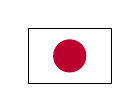
\begin{tikzpicture}
		\filldraw[draw=black,fill=white] (0,0) rectangle (3em,2em);
		\fill[JapanRed] (1.5em,1em) circle[radius=0.6em];
	\end{tikzpicture}\\
\end{tabular}\\
\begin{tabular}{p{0.4\textwidth}p{0.5\textwidth}}
	\textbf{Ecole Polytechnique} & \\
	$\rightarrow$ Master & \\
	\textsc{David Quéré} & \\
	& \textbf{University of Tokyo} (2005--2012)\\
	& \textsc{Hajime Tanaka}\\
	& Master \hfill$\Rightarrow$ \textit{E.P.L.} (2010)\\
	& PhD \hfill$\Rightarrow$ \textit{Nature Comm.} (2012)\\ 
	&\hfill\textit{Soft Matter} (2013)\\
	& Post-doc \hfill$\Rightarrow$ \textit{J. Chem. Phys.} (2013)\\ 		
	&\hfill\textit{Chem. Comm.} (2013)\\
	\textbf{E.N.S. Lyon} (09/2012--) & \\
	\textsc{Sébastien Manneville}& \\
	Post-doc&\\
\end{tabular}
\end{frame}
%\tikzset{external/force remake=false}

%\tikzset{external/force remake=true}
\begin{frame}{Mechanical response of of protein gels}
\begin{block}{A brittle fracture analogue to the one of solids}
\begin{columns}[T]
\column{0.2\textwidth}
\includegraphics[width=\textwidth]{TEM_yaourt_5um}
\column{0.25\textwidth}
{\scriptsize Kalab 1983}
\begin{itemize}
\item rheology
\item velocimetry
\item visualisation
\end{itemize}
\column{0.5\textwidth}
{\footnotesize reversible creep + irreversible fractures}\\
\tikzsetnextfilename{yaourt_creep}\begin{tikzpicture}
\begin{loglogaxis}[%
	tiny,
	name=g,
	axis background/.style={fill=white},
	width=0.5\textwidth+1em,
	xlabel={time (s)},
	ylabel={deformation}, ymin=0.1, ymax=2,
	ytick={0.1,0.2,0.4,0.8,1.6},
	yticklabels={0.1,0.2,0.4,0.8,1.6},
	extra tick style={grid=major},
	extra y ticks={1}, extra y tick labels={},%
	label shift=-0.5em, 
	no marks,
	]
	\addplot+[orange!50!red] table {Y39_1000Pa.txt} node[pos=0.58,left,font=\tiny,inner sep=2pt] (b) {\SI{1000}{\pascal}};
	\addplot+[red] table {Y32_550Pa.txt};
	\addplot+[red!75!black] table {Y25_400Pa.txt};
	\addplot+[red!50!black] table {Y38_300Pa.txt};
	\addplot+[red!25!black] table {Y27_200Pa.txt} node[pos=0.2,right,font=\tiny,inner sep=2pt] (a) {\SI{200}{\pascal}};
\end{loglogaxis}
\node[below right=0 and 5pt of g.north east,inner sep=0] (f1) {\includegraphics[width=0.25\textwidth-5pt]{yaourt_fractures_small.jpg}};
\node[right=5pt of f1,inner sep=0] (f2) {\includegraphics[width=0.25\textwidth-5pt]{yaourt_fractures_final.jpg}};
%\node[above right=0 of g.outer north west, font=\footnotesize, inner sep=0] {};
\path (f1.south) -- (f2.south) node[midway, below, font=\tiny] {Couette cell};
\end{tikzpicture}
\end{columns}
{\footnotesize Leocmach, Perge, Divoux \& Manneville \textit{ArXiv 1401.8234}}
\end{block}

\begin{block}{Syn\ae{}resis and confined wrinkling cascade}
\begin{columns}
\column{0.55\textwidth}
\begin{itemize}
\item solvent expulsion (pH $\rightarrow$ pI)
\item swelling (pH < pI)
\end{itemize}
\column{0.3\textwidth}
\tikzsetnextfilename{yaourt_cut}\begin{tikzpicture}
	\matrix[matrix of nodes, inner sep=0, row sep=1pt]{
\includegraphics[width=\columnwidth]{coupe_av10_cas8_t000.png}\\
\includegraphics[width=\columnwidth]{coupe_av10_cas8_t014.png}\\
\includegraphics[width=\columnwidth]{coupe_av10_cas8_t053.png}\\
\includegraphics[width=\columnwidth]{coupe_av10_cas8_t078.png}\\
%\includegraphics[width=\columnwidth]{coupe_av10_cas8_t088.png}\\
};
\end{tikzpicture}
\end{columns}
\tikzsetnextfilename{yaourt_times}\begin{tikzpicture}
	\matrix[matrix of nodes, inner sep=0, column sep=0.01\textwidth, row sep=0.5em, ampersand replacement=\&] (m){
	%33 min \& 38 min \& 43 min \& 48 min \& 1h \& 1h15 \& 2h30\\
	\includegraphics[width=0.13\textwidth]{prise_0100_color.jpg}\&
	\includegraphics[width=0.13\textwidth]{prise_0130_color.jpg}\&
	\includegraphics[width=0.13\textwidth]{prise_0160_color.jpg}\&
	\includegraphics[width=0.13\textwidth]{prise_0190_color.jpg}\&
	\includegraphics[width=0.13\textwidth]{prise_0250_color.jpg}\&
	\includegraphics[width=0.13\textwidth]{prise_0360_color.jpg}\&
	\includegraphics[width=0.13\textwidth]{prise_0799_color.jpg}\\
	\includegraphics[width=0.13\textwidth]{cas3p2_fluo0p8_GDL4_2_t047_crop_resized.jpg}\&
	\includegraphics[width=0.13\textwidth]{cas3p2_fluo0p8_GDL4_2_t056_crop_resized.jpg}\&
	\includegraphics[width=0.13\textwidth]{cas3p2_fluo0p8_GDL4_2_t065_crop_resized.jpg}\&
	\includegraphics[width=0.13\textwidth]{cas3p2_fluo0p8_GDL4_2_t074_crop_resized.jpg}\&
	\includegraphics[width=0.13\textwidth]{cas3p2_fluo0p8_GDL4_2_t092_crop_resized.jpg}\&
	\includegraphics[width=0.13\textwidth]{cas3p2_fluo0p8_GDL4_2_t125_crop_resized.jpg}\&
	\includegraphics[width=0.13\textwidth]{cas3p2_fluo0p8_GDL4_2_t260_crop_resized.jpg}\\
	};
	\draw[ultra thick] ++(m-1-1.south west) -- ++(0.023\textwidth,0) node[pos=0,below right=2pt and 0,inner sep=0,font=\tiny]{\SI{1}{\milli\metre}};
	\draw[ultra thick] ++(m-2-1.south west) -- ++(0.1\textwidth,0) node[pos=0,below right=2pt and 0,inner sep=0,font=\tiny]{\SI{1}{\milli\metre}};
	\end{tikzpicture}
\end{block}
\end{frame}
%\tikzset{external/force remake=false}

\begin{frame}[plain]
	\tableofcontents[hidesubsections]
	{\footnotesize Leocmach \& Tanaka \textit{Nature Communications} 3, 974 (2012).}
\end{frame}



%\include{current_slide}

\section{Supercooled liquids and the glass transition}
\tikzsetnextfilename{cooling}
\begin{frame}{From liquid to glass}
	\begin{columns}
	\column{0.6\textwidth}
	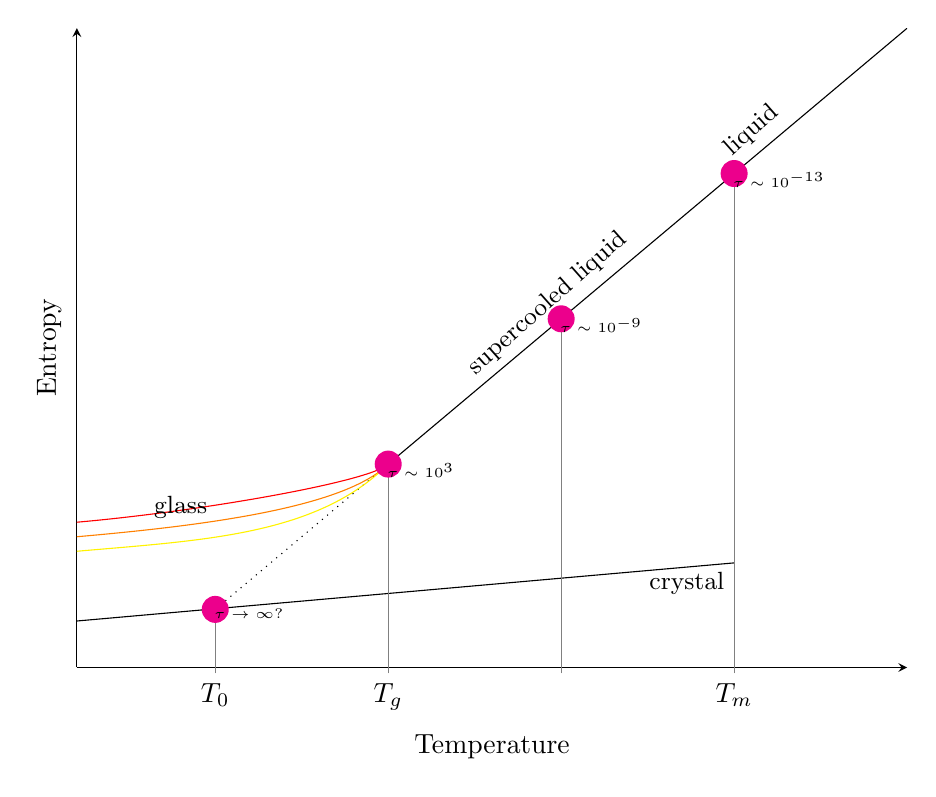
\begin{tikzpicture}[
		temp/.style={circle, inner sep=0.01\columnwidth, outer sep=0, fill=magenta},%
		label position=below right, label distance=-0.03\columnwidth,%
		]
	\begin{axis}[%
		width=\columnwidth, height=0.8\columnwidth,%
		xlabel=Temperature, xmin=0, xmax=1.2, axis x line=bottom, xtick=\empty,%
		extra x ticks={0.2, 0.45, 0.7, 0.95}, extra x tick labels={$T_0$, $T_g$,,$T_m$},%
		ylabel=Entropy, ymin=0.1, ymax=1.2, axis y line=left, ytick=\empty, ylabel near ticks,%
		]
		\draw (axis cs:0, 0.18) -- (axis cs:0.95, 0.28);
		\draw (axis cs:0.45, 0.45) -- (axis cs:1.2,1.2);
		\draw[dotted] (axis cs:0.2, 0.2)-- (axis cs:0.45, 0.45);
		\draw[help lines] (axis cs:0.2, 0)-- (axis cs:0.2, 0.2);
		\draw[help lines] (axis cs:0.45, 0)-- (axis cs:0.45, 0.45);
		\draw[help lines] (axis cs:0.7, 0)-- (axis cs:0.7, 0.7);
		\draw[help lines] (axis cs:0.95, 0)-- (axis cs:0.95, 0.95);
		\draw[red] (axis cs:0.45, 0.45) to [out=225, out looseness=0.2, in=5] (axis cs:0,0.35);
		\draw[orange] (axis cs:0.45, 0.45) to [out=225, out looseness=0.5, in=5] (axis cs:0,0.325);
		\draw[yellow] (axis cs:0.45, 0.45) to [out=225, out looseness=0.8, in=5] (axis cs:0,0.3);
		\node[temp, label=\tiny{$\tau\sim10^{-13}$}] at (axis cs:0.95, 0.95) {};
		\node[temp, label=\tiny{$\tau\sim10^{-9}$}] at (axis cs:0.7, 0.7) {};
		\node[temp, label=\tiny{$\tau\sim10^{3}$}] at (axis cs:0.45, 0.45) {};
		\node[temp, label=\tiny{$\tau\rightarrow\infty$?}] at (axis cs:0.2, 0.2) {};
		\node[above, anchor=south] at (axis cs:0.15, 0.34) (gl) {\small{glass}};
		\node[above, anchor=south, rotate=41.5] at (axis cs:0.7,0.7) {\small{supercooled liquid}};
		\node[above, anchor=south west, rotate=41.5] at (axis cs:0.95,0.95) {\small{liquid}};
		\node[below, anchor=north east] at (axis cs:0.95,0.28) {\small{crystal}};
	\end{axis}
	\end{tikzpicture}
	%\begin{footnotesize}\citet{cavagna2009supercooled}\end{footnotesize}
	\column{0.4\textwidth}
	\begin{itemize}
		\item Avoid crystallisation
		\item Slowing down by \alert{many} orders of magnitude
		\item A different type of solid: Glass
	\end{itemize}
	\end{columns}
	\begin{itemize}
		\item Kinetic glass transition $T_g$
		\item Not a thermodynamic transition but a dynamical arrest
	\end{itemize}
\end{frame}

\begin{frame}{Glass are amorphous}
	\begin{columns}
	\column{0.5\textwidth}
	Static structure factor
	\centering
	\includegraphics[width=\columnwidth]{sq_kob}
	
	{\footnotesize\citet{Kob2002}}
	
	\column{0.5\textwidth}
	While dynamics changes by 4 orders of magnitude
	\begin{itemize}
		\item Almost no change in positional order
		\item No characteristic length scale diverging toward $T_g$ or $T_0$
		\item $\neq$ critical phenomena
	\end{itemize}
	\end{columns}
\end{frame}

\tikzsetnextfilename{msd_kob}
\begin{frame}{Dynamics of supercooled liquids}

	{\footnotesize\citet{kob1995tmc}}
	\begin{columns}
	\column{0.4\textwidth}
	\centering
	\begin{tikzpicture}
		\node[above right] {\includegraphics[width=0.95\columnwidth]{msd_kob}};
		\node at(0.9\columnwidth, 0.65\columnwidth) {$\alpha$};
		\node at(0.2\columnwidth, 0.35\columnwidth) {$\beta$};
	\end{tikzpicture}
	
	\includegraphics[width=\columnwidth]{cage_weeks}\\
	\column{0.55\textwidth}
	%Mean square displacement\\
	\begin{block}{Two step relaxation}
	\begin{itemize}
		\item A plateau appears
		\item $\beta$-relaxation does not change
		\item The length of the plateau changes\\ $\Rightarrow$ slowing down by many orders of magnitude
	\end{itemize}
	\end{block}
	\begin{block}{The cage theory}
	\begin{itemize}
		\item Hopping between cages $\ll\sigma$
		\item Is the hopping probability really uniform?
	\end{itemize}
	\end{block}
	\end{columns}
	{\footnotesize\citet{weeks2002pcr}}
\end{frame}

\begin{frame}{Dynamic is heterogeneous}
	\begin{columns}
	\column{0.4\textwidth}
	Fast and slow regions exist at intermediate times.
	\begin{center}
	\includegraphics[width=\columnwidth]{dh_perera}\\
	{\footnotesize\citet{Perera1999}}
	\end{center}
	
	\column{0.6\textwidth}
	\begin{center}
	{\footnotesize\citet{Lacevic2003}}\\
	\includegraphics[width=0.7\columnwidth]{xi4_lacevic}
	\end{center}
	\begin{itemize}
		\item Spatial correlation of the fluctuations of the dynamics.
		\item Extract a dynamical correlation length
		\item Grows toward the glass transition
	\end{itemize}
	\end{columns}
\end{frame}

\tikzsetnextfilename{dynamic_vs_static}
\begin{frame}{Dynamic vs static ?}\usebeamercolor{block title}
\begin{flushright}
	\begin{tikzpicture}[concept/.style={scale=0.75, circle, font=\small, align=center, draw=bg, fill=bg, text width=6em, inner sep=0em}]
		\node[concept] (root2) {criticality};
		\node[below left=of root2, concept] (d2) {growing \alert{static} length scale};
		\node[below right=of root2, concept] (s2) {slow down of global dynamics};
		\path (root2) to[circle connection bar switch color=from (bg) to (bg)] (d2);
		\path (root2) to[circle connection bar switch color=from (bg) to (bg)] (s2);
		\draw [thick, fg, ->] (d2) to [bend right] (s2);		
		
		\node[below right=0.15\textwidth and 0.3\textwidth of root2, concept] (root) {glass transition};
		\node[below right=of root, concept] (s) {slow down of dynamics};
		\node[below=of root, concept] (d) {growing \alert{dynamic} length scale};
		\node<2>[below left=of root, concept] (sta) {growing \alert{static} length scale};
		\path (root) to[circle connection bar switch color=from (bg) to (bg)] (d);
		\path (root) to[circle connection bar switch color=from (bg) to (bg)] (s);
		\path<2> (root) to[circle connection bar switch color=from (bg) to (bg)] (sta);
		\draw[thick, dashed, fg, ->] (d) to [bend right] (s);
		\draw<2>[thick, dashed, fg, ->] (sta) to [bend right] (d);
	\end{tikzpicture}
\end{flushright}
\end{frame}

\begin{frame}{Static cause to dynamic heterogeneities}
	\begin{columns}
	\column{0.5\textwidth}
	\centering
	\includegraphics[width=\columnwidth]{propensity}
	\column{0.5\textwidth}
	{\footnotesize\citet{Widmer-Cooper2005}}
	\begin{itemize}
		\item $N$ runs from the same initial configuration
		\item Average out the influence of initial dynamics
		\item Propensity to displacement
		\item Predict fast/slow \alert{regions} ($>$~individual particle)\\{\footnotesize\citet{Berthier2007}}
	\end{itemize}
	\end{columns}
	
	\bigskip$\Rightarrow$ Glass transition may have a structural cause
\end{frame}

\tikzsetnextfilename{pentagons}
\begin{frame}{Candidates of structural order}
\small{Without long-ranged positional order}
\begin{columns}
\column{0.5\textwidth}
\begin{block}{Locally favoured structure (LFS) of the liquid}
Cannot fill space because of geometrical frustrations

\centering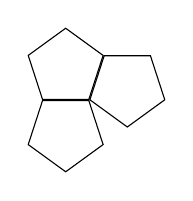
\begin{tikzpicture}[pen/.style={regular polygon, regular polygon sides=5, draw, minimum size=1cm}]
	\node[pen] (base) {};
	\node[pen,anchor=south, rotate=180] at (base.side 3) {};
	\node[pen,anchor=south, rotate=-108] at (base.side 4) {};
\end{tikzpicture}
\end{block}
Example: Icosahedron
\column{0.5\textwidth}
\centering\includegraphics[width=0.5\textwidth]{d20.png}

\includegraphics[width=0.5\textwidth]{ico_13}
\end{columns}
\end{frame}

\tikzsetnextfilename{hexagons}
\begin{frame}{Candidates of structural order}
\small{Without long-ranged positional order}
\begin{columns}
\column{0.5\textwidth}
\begin{block}{Influence of the crystal}
Cannot fill space because
\begin{itemize}
	\item Energy barrier
	\item Other structures locally more stable
	\item Kinetic barrier
	\item Size polydispersity
\end{itemize}
\end{block}
Example: Depends on the underlying crystal structure
\column{0.5\textwidth}
	\centering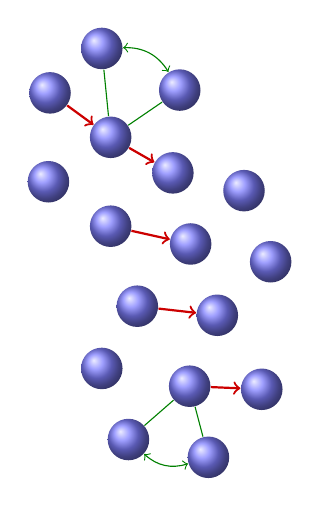
\begin{tikzpicture}[scale=0.2, rotate=-90]
		\tikzset{particle/.style={circle, ball color=blue!50!white, inner sep=0, minimum size=1.5em}}
		\tikzset{ar/.style={->, draw=red!80!black, thick}}
		\node[particle] at (14.356, 47.436) (a) {};
		\node[particle] at (17.000, 52.387) (b) {};
		\node[particle] at (20.000, 48.000) (c) {};
		\node[particle] at (17.178, 44.149) (d) {};
		\node[particle] at (22.258, 51.951) (e) {};
		\node[particle] at (22.822, 44.049) (f) {};
		\node[particle] at (23.387, 56.467) (g) {};
		\node[particle] at (27.902, 58.160) (g1) {};
		\node[particle] at (26.773, 53.080) (h) {};
		\node[particle] at (25.644, 48.000) (i) {};
		\node[particle] at (31.300, 54.773) (j) {};
		\node[particle] at (30.724, 49.693) (k) {};
		\node[particle] at (36.000, 57.596) (k1) {};
		\node[particle] at (35.804, 53.016) (l) {};
		\node[particle] at (34.676, 47.436) (m) {};
		\node[particle] at (40.320, 54.209) (n) {};
		\node[particle] at (39.191, 49.129) (o) {};
		\path[ar] (d) edge (c);
		\path[ar] (c) edge (e);
		\path[ar] (i) edge (h);
		\path[ar] (k) edge (j);
		\path[ar] (l) edge (k1);
		\draw[green!50!black] (a) -- (c) -- (b);
		\path[green!50!black,<->] (a) edge [bend left] (b);
		\draw[green!50!black] (n) -- (l) -- (o);
		\path[green!50!black,<->] (n) edge [bend left] (o);
	\end{tikzpicture}
\end{columns}
\end{frame}

\begin{frame}{Different structural cause $\Rightarrow$ different theory}
\begin{columns}[T]
\column{0.5\textwidth}
\structure{Liquid's order}
\begin{itemize}
	\item Spin-glass type\\{\footnotesize\citet{steinhardt1983boo}}
	\item Frustration-limited domain\\{\footnotesize\citet{tarjus2005fba}}
\end{itemize}
Icosahedral domain size\\
Defect size

\column{0.5\textwidth}
\structure{Crystal's order}
\begin{itemize}
	\item Tow order parameters\\{\footnotesize\citet{TanakaGJPCM}}
\end{itemize}

\bigskip
Bond order coherence length
\end{columns}
\begin{columns}
\column{0.5\textwidth}
\rotatebox{90}{\footnotesize \citet{Dzugutov2002}}
\includegraphics[width=0.5\columnwidth]{Dzugutov_LFS}
\column{0.5\textwidth}
\begin{tabular}{cc}
\resizebox{0.45\columnwidth}{!}{\input{kawa_nm_psi6.pdf_tex}} & \resizebox{0.45\columnwidth}{!}{\input{kawa_nm_msd.pdf_tex}} \\ 
$\Psi_6$ & $\Delta r^2$ \\ 
\end{tabular}
{\footnotesize\citet{tanaka2010critical}}
\end{columns}
\end{frame}

\begin{frame}{"Crystal" is \ldots}
\ldots the symmetry breaking phase, avoided \alert{by definition} to get the supercooled liquid.
\begin{itemize}
	\item A classical crystal (\textsc{fcc, hcp, bcc}, \ldots)
\end{itemize}
\begin{columns}[T]
	\column{0.5\textwidth}
	\centering
	\begin{itemize}\item A quasi-crystal\end{itemize}
	\includegraphics[height=0.5\columnwidth]{Ho-Mg-ZnQuasicrystal.jpg}\\
	{\footnotesize\citet{Doye2003}}
	\column{0.5\textwidth}
	\centering
	\begin{itemize}\item A Frank-Kasper phase\end{itemize}
	\includegraphics[height=0.5\columnwidth]{frankkasper.png}\\
	{\footnotesize\citet{Pedersen2010, Coslovich2011}}
\end{columns}

\bigskip
$\Rightarrow$ "Crystal" may contain icosahedral motif
\end{frame}

\begin{frame}{Slow icosahedral cluster means \dots}
\dots \alert{nothing} if the (quasi)crystalline state of the system has icosahedral motif.
\begin{itemize}
	\item Dodecagonal quasi-crystal for Dzugutov system\\{\footnotesize\citet{Doye2003}}
	\item Frank-Kasper phase for Wangstr\"om mixture\\{\footnotesize\citet{Pedersen2010, Coslovich2011}}
\end{itemize}

\begin{block}{We need a system}
\begin{itemize}
	\item With a known crystalline state $\nsupseteq$ icosahedral motif
	\item Exhibiting icosahedral order
\end{itemize}
\centering$\Longrightarrow$ Hard spheres
\end{block}
\end{frame}

\section{Hard spheres colloids tracked by confocal microscopy}
\begin{frame}{Hard spheres and colloids}
	\begin{textblock*}{0.6\textwidth}(10mm,88mm)
		\simplephasediagram{}%
	\end{textblock*}
	The volume fraction $\phi$ is like an inverse temperature.
	\bigskip
	\def\svgwidth{\textwidth}\input{phase_diagram.pdf_tex}
	
	\bigskip
	Well approximated by sterically stabilised colloids\\
	\begin{footnotesize}\citet{pusey1987ogt}\end{footnotesize}
\end{frame}

\tikzsetnextfilename{sem_hist}
\begin{frame}{Our colloids}
	\begin{columns}
	\column{0.5\textwidth}
	\begin{center}
	\rotatebox{90}{\qquad \small{SEM image}}\includegraphics[width=0.8\columnwidth, height=0.6\columnwidth]{SEM}
	\end{center}
	\structure{Solvent}
	\begin{itemize}
		\item Cis-decalin
		\item Cyclohexylbromide
	\end{itemize}
	Matching
	\begin{itemize}
		\item Optical index
		\item Density (with $T$ control)
	\end{itemize}
	\column{0.5\textwidth}
	\begin{block}{PMMA particles}
		\begin{itemize}
			\item $\sigma \simeq \SI{3.3}{\micro\metre}$
			\item $\Delta \simeq 6\%$ not Gaussian
		\end{itemize}
		Hard spheres
		\begin{itemize}
			\item Sterically stabilized
			\item Salt to screen charges\\ (Debye length $<\SI{100}{\nano\metre}$)
		\end{itemize}
	\end{block}
	\begin{tikzpicture}
		\begin{axis}[%
			width=\columnwidth, height=0.6\columnwidth,%
			ybar,%
			ymin=0, ylabel={Size distribution},%
			xlabel={Sizes [\si{\micro\metre}]}
			]
		\usebeamercolor{palette primary}
		\addplot[ybar interval, fill=fg!50!white] file {SEM_size_distrib.txt};
		\end{axis}
	\end{tikzpicture}
	\end{columns}
\end{frame}

\tikzsetnextfilename{confocal}
\begin{frame}{Confocal microscopy}
	\begin{center}\begin{columns}[c]
	\column{0.4\textwidth}
	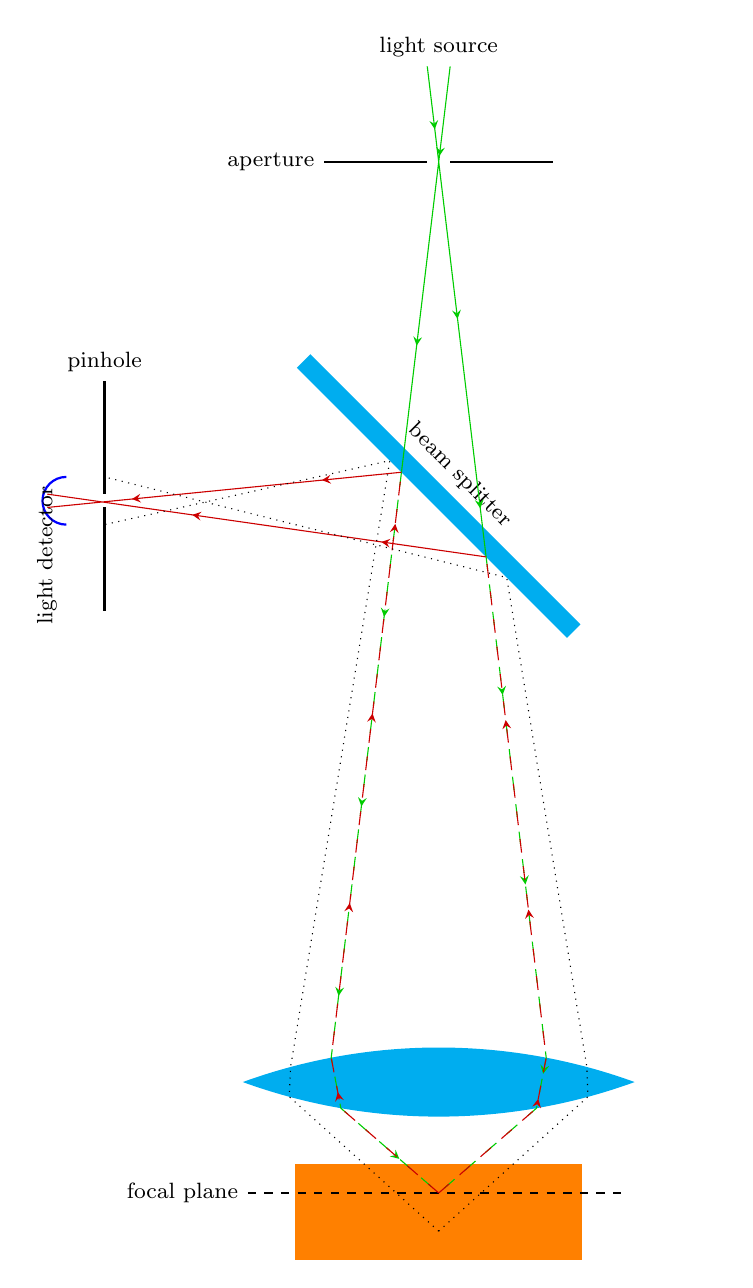
\begin{tikzpicture}[
		font=\footnotesize, 
		decoration={markings, mark=between positions 0.1 and 1 step 0.2\columnwidth with {\arrow{stealth}}},
	]
	\draw[thick] (-0.12\columnwidth,0) -- (-0.012\columnwidth,0) (0.012\columnwidth,0) -- (0.12\columnwidth,0);
	\node[left] at (-0.12\columnwidth,0) {aperture};
	\fill[name path=dichro, cyan, rotate around={-45:(0,-0.35\columnwidth)}]  (-0.2\columnwidth,-0.34\columnwidth) rectangle (0.2\columnwidth,-0.36\columnwidth) (0, -0.34\columnwidth) node[above, black, rotate=-45] {beam splitter};
	\draw[thick] (-0.35\columnwidth,-0.23\columnwidth) -- (-0.35\columnwidth,-0.348\columnwidth) (-0.35\columnwidth,-0.362\columnwidth) -- (-0.35\columnwidth,-0.47\columnwidth);
	\node[above] at (-0.35\columnwidth,-0.23\columnwidth) {pinhole};
	\fill[cyan] (0, -\columnwidth) arc (-90:-70:0.6\columnwidth) node (lensright) {} 
		arc (70:110:0.6\columnwidth) node (lensleft) {}
		arc (-110:-90:0.6\columnwidth);
	\path[name path=lensbottom] (lensleft) arc (-110:-70:0.6\columnwidth);
	\path[name path=lenstop] (lensright) arc (70:110:0.6\columnwidth);
	\fill[orange] (-0.15\columnwidth, -1.05\columnwidth) rectangle (0.15\columnwidth, -1.15\columnwidth);
	\draw[dashed] (-0.2\columnwidth, -1.08\columnwidth) -- (0.2\columnwidth, -1.08\columnwidth);
	\node[left] at (-0.2\columnwidth, -1.08\columnwidth) {focal plane};
	\node[above] at (0,0.1\columnwidth) {light source};
	\path[name path=iray1] (0.012\columnwidth, 0.1\columnwidth) -- (-0.12\columnwidth, -\columnwidth);
	\path[name path=iray2] (0, -1.08\columnwidth) -- (-0.15\columnwidth, -0.95\columnwidth);
	\path[name path=iray3] (-0.012\columnwidth, 0.1\columnwidth) -- (0.12\columnwidth, -\columnwidth);
	\path[name path=iray4] (0, -1.08\columnwidth) -- (0.15\columnwidth, -0.95\columnwidth);
	\draw[
		postaction={decorate}, green!80!black,
		name intersections={of=iray1 and dichro, by=x},
		name intersections={of=iray3 and dichro, by=y},
		]
		(0.012\columnwidth, 0.1\columnwidth) -- (x)
		(-0.012\columnwidth, 0.1\columnwidth) -- (y);
		
	\draw[
		postaction={decorate}, green!80!black, dashed, dash pattern=on 5pt off 5pt, dash phase=0pt,
		name intersections={of=iray1 and dichro, by=x}, 
		name intersections={of=iray1 and lenstop, by=a}, 
		name intersections={of=iray2 and lensbottom, by=b},
		name intersections={of=iray4 and lensbottom, by=c},
		name intersections={of=iray3 and lenstop, by=d},
		name intersections={of=iray3 and dichro, by=y},
		] 
		(x) -- (a) -- (b) -- (0, -1.08\columnwidth)
		(y) -- (d) -- (c) -- (0, -1.08\columnwidth);
	\draw[postaction={decorate}, red!80!black, 
		name intersections={of=iray1 and dichro, by=x}, 
		name intersections={of=iray3 and dichro, by=y},
		] 
		(x) -- (-0.41\columnwidth, -0.362\columnwidth) 
		(y) -- (-0.41\columnwidth, -0.348\columnwidth);
	\draw[postaction={decorate}, red!80!black, dashed, dash pattern=on 5pt off 5pt, dash phase=10pt,
		name intersections={of=iray1 and dichro, by=x}, 
		name intersections={of=iray1 and lenstop, by=a}, 
		name intersections={of=iray2 and lensbottom, by=b},
		name intersections={of=iray4 and lensbottom, by=c},
		name intersections={of=iray3 and lenstop, by=d},
		name intersections={of=iray3 and dichro, by=y},
		] 
		(0, -1.08\columnwidth) -- (b) -- (a) -- (x) 
		(0, -1.08\columnwidth) -- (c) -- (d) -- (y);
	\draw[thick, blue] (-0.39\columnwidth, -0.33\columnwidth) arc (90:270:0.025\columnwidth);
	\node[above left, rotate=90] at (-0.39\columnwidth, -0.33\columnwidth) {light detector};
	\path[name path=badray1] (0,0) -- (-0.18\columnwidth, -1.1\columnwidth);
	\path[name path=badray2] (0, -1.12\columnwidth) -- (-0.3\columnwidth, -0.85\columnwidth);
	\path[name path=badray3] (0,0) -- (0.18\columnwidth, -1.1\columnwidth);	
	\path[name path=badray4] (0, -1.12\columnwidth) -- (0.3\columnwidth, -0.85\columnwidth);
	\draw[dotted,
		name intersections={of=badray1 and dichro, by=x}, 
		name intersections={of=badray1 and lenstop, by=a}, 
		name intersections={of=badray2 and lensbottom, by=b},
		name intersections={of=badray4 and lensbottom, by=c},
		name intersections={of=badray3 and lenstop, by=d},
		name intersections={of=badray3 and dichro, by=y},
		] 
		(0, -1.12\columnwidth) -- (b) -- (a) -- (x) --  (-0.35\columnwidth, -0.38\columnwidth)
		(0, -1.12\columnwidth) -- (c) -- (d) -- (y) --  (-0.35\columnwidth, -0.33\columnwidth);
	\end{tikzpicture}
	\column{0.5\textwidth}
	\tikzsetnextfilename{confocal_slices}
	\begin{tikzpicture}
	\matrix[matrix of nodes, ampersand replacement=\&, nodes={anchor=center}]
	{
		$XY$ slice \& \includegraphics[width=0.5\columnwidth]{sliceXY} \\
		$XZ$ slice \& \includegraphics[width=0.5\columnwidth]{sliceXZ} \\
	};
	\end{tikzpicture}
	\end{columns}\end{center}
\end{frame}

\begin{frame}<3>{Particle tracking}
	\begin{columns}
	\column{0.6\textwidth}
	\only<1|handout:0>{\includegraphics[width=\columnwidth]{compare_image_tracked3D_0}}%
	\only<2|handout:0>{\includegraphics[width=\columnwidth]{compare_image_tracked3D_1}}%
	\only<3>{\includegraphics[width=\columnwidth]{compare_image_tracked3D_2}}\\
	\centering{\uncover<1,3>{Image}\uncover<3>{ $+$ }\uncover<2,3>{Tracked}}
	\column{0.4\textwidth}
	\footnotesize{\citet{Crocker1996}}	
	
	\bigskip
	
	\begin{itemize}
		\item All particles are tracked
		\item Only particles are tracked
		\item Coordinates are known within\\
			$\SI{0.1}{pixels} \approx \sigma/100 \approx \SI{30}{\nano\metre}$
		\item \alert{new}: arbitrary size distribution
		\item \alert{new}: sizes measured \emph{in situ}
	\end{itemize}
	\end{columns}
\end{frame}


\tikzsetnextfilename{hist_SEM_vs_multiscale}
\begin{frame}{Multiscale tracking}
	\centering
	\begin{tikzpicture}
	\begin{axis}[%
		name=hist2,
		width=0.8\columnwidth, height=0.6\columnwidth,%
		xmin=1, xmax=5,
		ylabel={Size distribution},
		ymin=0, yticklabel=\empty, ylabel near ticks,%
		legend style={legend pos=north west},
		no marks,%
		]
		\addplot[ybar, ybar interval, area legend, gray!50, fill=gray!50] file {SEM_size_distrib.txt} \closedcycle;
		\legend{\textsc{sem}}
		\addplot+[blue,dashed] table[x expr ={2*\thisrow{r}}, y expr ={5.5*\thisrow{all}}] {all_ico_icongb_mrco_X.rdist};
		\addlegendentry{In situ};
		\addplot+[red] table [x expr ={2*\thisrow{r}/1.25}, y expr ={5.5*\thisrow{all}}] {all_ico_icongb_mrco_X.rdist};
		\addlegendentry{In situ*0.8};
		\draw[->, ultra thick] (axis cs:3.15,3) -- (axis cs: 3.9, 3) node[midway, above] {swelling};%
	\end{axis}
	\end{tikzpicture}%
	\includegraphics[width=0.2\columnwidth]{comp2D3D_crop}
	
	{\footnotesize Leocmach \& Tanaka \textit{Soft Matter} 9, 1447--1457 (2013).}
\end{frame}


\begin{frame}{Glassy dynamics}
	\begin{textblock*}{0.6\textwidth}(10mm,88mm)
		\simplephasediagram{}%
	\end{textblock*}
	From the tracked trajectories
	\tikzsetnextfilename{glassy_dynamics}%
	\begin{tikzpicture}
		\pgfplotsset{fitc/.style={solid, no markers, forget plot, domain=1:1e4}}
		\pgfplotsset{every axis/.append style={width=0.48\textwidth}}
		\pgfplotsset{cycle list name=grade5}
		\begin{axis}[%
			at={(0,0)},
			height=0.33\textwidth, %
			xlabel=$t/\tau_B$, xmode=log,%
			ylabel=\sffamily{Self ISF}, ymin=0,%
			legend style={at={(0,-0.5)}, anchor=north west},
			reverse legend,
			]
			\addplot+[fitc] {0.943 * exp(-(x/4.60)^0.72)};
			\addplot+[only marks] file {LS3954.isf};
			\addplot+[fitc] {0.901 * exp(-(x/10.78)^0.72)};
			\addplot+[only marks] file {LS4446.isf};
			\addplot+[fitc] {0.894 * exp(-(x/15.51)^0.70)};
			\addplot+[only marks] file {LS4582.isf};
			\addplot+[fitc] {0.876 * exp(-(x/60.18)^0.60)};
			\addplot+[only marks] file {LS5079.isf};
			\addplot+[fitc] {0.787 * exp(-(x/2408.)^0.70)};
			\addplot+[only marks] file {go1.isf};
			\addlegendimage{legend image code/.code={\node[right] {$\phi\;\pm$};}};
			\legend{$0.497$, $0.535$, $0.540$, $0.555$, $0.575$, $0.003$};
		\end{axis}
		\pgfplotsset{fitc/.style={no markers, forget plot, domain=0.3:3}}
		\begin{semilogxaxis}[%
			at={(0.49\textwidth,0)},
			height=0.33\textwidth, %
			xlabel=$t/\tau_B$,%
			xmin=1, xmax=1e4,%
			ylabel=$\alpha_2(t)$,%
			only marks,%
			]
			\addplot file {LS3954.ngp};
			\addplot file {LS4446.ngp};
			\addplot file {LS4582.ngp};
			\addplot file {LS5079.ngp};
			\addplot file {go1.ngp};
		\end{semilogxaxis}
		\pgfplotsset{cycle list name=black white}
		\tikzset{every mark/.append style={scale=1.2}}
		\begin{axis}[%
			at={(0.49\textwidth,-0.3\textwidth)},
			height=0.33\textwidth, %
			xlabel=$\phi$,%
			xtick={0.5,0.52,...,0.6},%
			ylabel=$\tau_\alpha/\tau_B$, ymode=log, %
			cycle list={{black, mark=*},{black, mark=square}},%
			]
			\addplot+[mark=none, forget plot, domain=0.49:0.58] {exp(0.28970401*x/(0.59841615-x))};
			\addplot+[only marks] table[x index=0, y index=1]{xi_phi.dat};
			\addplot+[only marks, every mark/.append style={draw=gray, scale=1.2}] table[x index=0, y index=4]{xi_phi.dat};
			\node at (rel axis cs:0,1) (a) {};
		\end{axis}
	\end{tikzpicture}
\end{frame}


\begin{frame}{Dynamic heterogeneities}
\begin{textblock*}{0.6\textwidth}(10mm,88mm)
		\simplephasediagram{}%
	\end{textblock*}
\begin{columns}
	\column{0.4\textwidth}
	Slow particles
	\includegraphics[width=\columnwidth]{cgsd_2tau.png}
	\column{0.6\textwidth}
	\tikzsetnextfilename{dynhet}%
	\begin{tikzpicture}
		\begin{loglogaxis}[%
			anchor=outer south,
			title={Four-point structure factor},
			width=0.9\textwidth,
			height=0.5\textwidth, %
			xlabel={$q\xi_4$}, ylabel={$S_4(q)/\chi_4$},
			cycle list name=grade5,%
			xmin=0.25, xmax=5, ymin=0.05,%
			xtick={0.5, 1, 2, 4},
			xticklabel=\pgfmathparse{exp(\tick)}%
				\pgfmathprintnumber{\pgfmathresult},
			%legend pos=south west, reverse legend,
			]
			\addplot+[only marks] table[x expr={\thisrowno{0}*0.703}, y expr={\thisrowno{1}/0.634}] {LS3954.S4};
			\addplot+[only marks] table[x expr={\thisrowno{0}*0.804}, y expr={\thisrowno{1}/0.744}] {LS4446.S4};
			\addplot+[only marks] table[x expr={\thisrowno{0}*0.835}, y expr={\thisrowno{1}/0.778}] {LS4582.S4};
			\addplot+[only marks] table[x expr={\thisrowno{0}*1.017}, y expr={\thisrowno{1}/1.011}] {LS5079.S4};
			\addplot+[only marks] table[x expr={\thisrowno{0}*1.959}, y expr={\thisrowno{1}/2.950}] {go1.S4};
			\addplot+[black, no markers, forget plot, domain=0.3:3] {1/(1+x^2)};
		\end{loglogaxis}
		\pgfplotsset{cycle list name=black white}
		\tikzset{every mark/.append style={scale=1.2}}
		\begin{axis}[%
			anchor=outer north,
			title={Growing dynamic length scale},
			%at={(0.1\textwidth,-0.6\textwidth)},
			width=0.6\textwidth, %
			xlabel=$\phi$, xmin=0.49, xmax=0.58, xlabel near ticks,%
			xtick={0.5,0.52,...,0.6},%
			ylabel=$\xi_4$, ymax=2.5,
			ytick={0.5,1,1.5,2},
			ylabel near ticks,%
			]
			\addplot+[mark=none, forget plot, domain=0.49:0.58] {0.216 * (0.6/x-1)^(-2.0/3.0)};
			\addplot+[only marks, mark=square, every mark/.append style={draw=gray, scale=1.2},] table[x index=0, y expr=\thisrowno{5}]{scale.xi};
		\end{axis}
	\end{tikzpicture}
\end{columns}
\end{frame}

\section[Structure]{Structure identification}
\tikzsetnextfilename{spherical_harmonics}
\begin{frame}[label=local_sym_sh]{Local symmetry and spherical harmonics}
	\begin{columns}
	\column{0.25\textwidth}
	\begin{center}
	\includegraphics[width=\columnwidth]{fig_espci/hexagons}
	\end{center}
	\column{0.75\textwidth}
	\begin{tikzpicture}
		\matrix (mat) [%
			matrix of nodes, ampersand replacement=\&, nodes={anchor=center},%
			row 1/.style={font=\tiny}, row 4/.style={font=\tiny}
			]
		{
			$\ell=6, m=0$ \& \& $\ell=6, m=5$ \& \& Icosahedron\\
			\includegraphics[width=0.25\columnwidth]{sh6-0} \& %
			$+$ \& %
			\includegraphics[width=0.25\columnwidth]{sh6-5} \& %
			$=$ \& %
			\includegraphics[width=0.25\columnwidth]{ico_13} \\
			\includegraphics[width=0.25\columnwidth]{sh6-3} \& %
			$+$ \& %
			\includegraphics[width=0.25\columnwidth]{sh6-6} \& %
			$=$ \& %
			\includegraphics[width=0.25\columnwidth]{fcc_13} \\
			$\ell=6, m=3$ \& \& $\ell=6, m=6$ \& \& \textsc{fcc}\\
		};
	\end{tikzpicture}
	\end{columns}
	\begin{itemize}
		\item The orientation changes $\Rightarrow$ No positional order
		\item The local angles stay the same $\Rightarrow$ Bond orientational order
	\end{itemize}
	{\footnotesize\citet{steinhardt1983boo}}
\end{frame}


\begin{frame}<1-3>{Second-shell bond orientational order}
	\begin{textblock*}{0.6\textwidth}(10mm,88mm)
		\only<2->{\simplephasediagram{%
			\node<2-> at (0.576,0) [xp marker, fill=green!50!black] {};%
			\node<3-> at (0.497,0) [xp marker, fill=green!50!black] {};
			}}%
	\end{textblock*}
	\begin{columns}[b]
	\column{0.5\textwidth}
	\alt<-2>{\tikzsetnextfilename{Q4Q6_maps}}{\tikzsetnextfilename{Q4Q6phi3954}}%
	\begin{tikzpicture}
		\node (bcc) {\includegraphics[width=0.25\columnwidth]{bcc_15}};
		\node[right=0 of bcc] (hcp) {\includegraphics[width=0.25\columnwidth]{hcp_13}};
		\node[right=0 of hcp] (fcc) {\includegraphics[width=0.25\columnwidth]{fcc_13}};
		\begin{axis}[%
			anchor=north east, at=(fcc.south east),%
			width=\columnwidth, height=\columnwidth,%
			ylabel={$Q_6$}, xlabel=$Q_4$,%
			xmin=0,xmax=0.22,%
			ymin=0, ymax=0.6,%
			enlargelimits=false,axis on top,
			extra tick style={grid=major},%
			extra y ticks={\Qstar}, extra y tick labels={},%
			xticklabel={$\pgfmathprintnumber[fixed,precision=2]{\tick}$}
			] 
		\alt<-2>{\addplot graphics
		[xmin=0,xmax=0.2,ymin=0,ymax=0.6]
		{lechner_Q4Q6.png};
		\matrix[
			matrix of nodes, ampersand replacement=\&, matrix anchor=south east,%
			nodes={inner sep=0.25em, anchor=west},%
			column 1/.style={circle},%
			] at (rel axis cs:1,0)
		{
			|[fill=black]| \& \textsc{bcc}\\
			|[fill=orange!80!black]| \& \textsc{fcc}\\
			|[fill=green!80!black]| \& \textsc{hcp}\\
			|[fill=blue!80!black]| \& aperiodic\\
		};
		}{\addplot graphics
		[xmin=0,xmax=0.2,ymin=0,ymax=0.6]{Q4Q6phi3954.png};}
		
		\node at (axis cs:0.1909, 0.5745) (infcc){};
		\node at (axis cs:0.0972222, 0.484762) (inhcp){};
		\node at (axis cs:0.0363696, 0.510688) (inbcc){};
		\end{axis}
		\draw[->, black] (bcc) -- (inbcc);
		\draw[->, green!80!black] (hcp) -- (inhcp);
		\draw[->, orange!80!black] (fcc) -- (infcc);
	\end{tikzpicture}
	\column{0.5\textwidth}
	\alt<1>{%
	{\footnotesize\citet{lechner2008}}

	\bigskip	
	
	\begin{itemize}
		\item $Q_\ell$ is the strength of the $\ell$-fold symmetry
		\item Very good at telling apart
			\begin{itemize}
				\item aperiodic structures
				\item locally periodic
			\end{itemize}
		\item Differentiate between crystal structures
	\end{itemize}
	
	\bigskip	
	%
	}{\tikzsetnextfilename{Q4Q6}
	\begin{tikzpicture}
		\begin{axis}[%
			width=\columnwidth, height=\columnwidth,%
			ylabel={$Q_6$}, xlabel=$Q_4$,%
			xmin=0,xmax=0.22,%
			ymin=0, ymax=0.6,%
			enlargelimits=false,axis on top,
			colormap={bw}{gray(0cm)=(1); gray(1cm)=(1); gray(10cm)=(0)},%
			colorbar sampled, colorbar horizontal, 
			colorbar style={%
				xlabel={per units of $Q_4\cdot Q_6$},% 
				xticklabels={$10^{1}$, $10^{2}$, $10^{3}$, $10^{4}$},%
				samples=6, xtick={ 0.20,0.4,0.6, 0.8},% 
				extra y ticks={},%
				/pgfplots/colorbar shift/.style={yshift=0.3cm},
				at={(parent axis.north)}, anchor=below south, width=0.9*\pgfkeysvalueof{/pgfplots/parent axis width},
				xticklabel pos=upper,%
				label style={font=\footnotesize},
				},%
			xticklabel={$\pgfmathprintnumber[fixed,precision=2]{\tick}$},%
			extra tick style={grid=major},%
			extra y ticks={\Qstar}, extra y tick labels={},%
			]
		\addplot graphics
		[xmin=0,xmax=0.2,ymin=0,ymax=0.6]
		{Q4Q6go1};
		\node [below] at (axis cs:0.1909, 0.5745) {\textsc{fcc}};
		\node [below] at (axis cs:0.0972222, 0.484762) {\textsc{hcp}};
		\node [below] at (axis cs:0.0363696, 0.510688) {\textsc{bcc}};
		\draw[->, white,thick] (axis cs:0.05, 0.15) to [out=60, in=220] (axis cs:0.125, 0.4);
		\end{axis}
	\end{tikzpicture}}
	\end{columns}
\end{frame}

\begin{frame}{Icosahedral order}
	\begin{textblock*}{0.6\textwidth}(10mm,88mm)
		\simplephasediagram{%
			\node at (0.576,0) [xp marker, fill=green!50!black] {};%
			\node at (0.497,0) [xp marker, fill=green!50!black] {};}
	\end{textblock*}
	\begin{columns}
	\column{0.5\textwidth}
	$w_6$
		\begin{itemize}
		\item first shell only
		\item sensitive to aperiodic
		\item icosahedral order stands out
		\end{itemize}
	\column{0.5\textwidth}
	\begin{block}{Two types of order}
		\begin{itemize}
		\item orthogonal
		\item incompatible
		\item mutual frustration
		\end{itemize}
	\end{block}
	\end{columns}
	\begin{center}\tikzsetnextfilename{w6Q6}
	\begin{tikzpicture}
		\pgfplotsset{
			extra tick style={grid=major},%
			every axis/.append style={%
				height=0.4\textwidth,
				ymin=0,ymax=0.6,%
				extra y ticks={\Qstar}, extra y tick labels={},%
				enlargelimits=false,axis on top,
				colormap={bw}{gray(0cm)=(1); gray(1cm)=(1); gray(10cm)=(0)},%
				colorbar sampled,%
				},%
		}
		\begin{groupplot}[
			group style={
				group size=2 by 1,%
				yticklabels at=edge left,%
				horizontal sep=0pt,%
				},%
			anchor=above north west,%
			width=0.38\textwidth,%
			xlabel=$10^2 \cdot w_6$,%
			xmin=-0.052,xmax=0.01,%
			extra x ticks={\wstar, -0.00782},%
			extra x tick labels={,},%
			xtick scale label code/.code={},%
			colorbar right, colorbar style={%
				samples=6, ytick={ 0.20,0.4,0.6, 0.8},% 
				yticklabels={$10^{1}$, $10^{2}$, $10^{3}$, $10^{4}$},%
				ylabel={per units of $w_6\cdot Q_6$},%
				extra x ticks={},%
				extra y ticks={},%
				label style={font=\footnotesize},
				},%
			]
		\nextgroupplot[ylabel={$Q_6$}, xtickmax=0,]
		\addplot graphics
		[xmin=-0.052,xmax=0.052,ymin=0,ymax=0.6]
		{u6Q6phi3954_scale};
		\node [above] at (axis cs:-0.04, \Qstar) {\footnotesize{$Q_6^*$}};
		%\node [anchor=north east] at (rel axis cs:1, 1) {\footnotesize{$\phi = 0.497 \pm 0.03$}};
		\node [left] at (axis cs:\wstar,0.4) {\footnotesize $w_6^*$};
		\node [right] at (axis cs:-0.00782,0.4) {\footnotesize $w_6^{dod}$};
		
		\nextgroupplot
		\addplot graphics
		[xmin=-0.052,xmax=0.052,ymin=0,ymax=0.6]
		{u6Q6go1_scale};
		\node at (axis cs:\wstar,0.6) (a) {};
		\node at (axis cs:-0.00782,0.6) (b) {};
		\node [below] at (axis cs:-0.0026, 0.5745) {\textsc{fcc}};
		\node [below, right] at (axis cs:-0.052, 0.05) {\textsc{Ico}};
		\draw[->, white,thick] (axis cs:-0.001, 0.15) to [out=90, in=275] (axis cs:-0.0015, 0.33);
		\draw[->, white,thick] (axis cs:-0.001, 0.15) to [out=180, in=30] (axis cs:-0.025, 0.12);
		
		\end{groupplot}
	\end{tikzpicture}\end{center}
\end{frame}

\section[Link with dynamics]{Link between structures and dynamics}
\begin{frame}{Bond order mobility}
	\begin{textblock*}{0.6\textwidth}(10mm,88mm)
		\simplephasediagram{\node at (0.576,0) [xp marker, fill=green!50!black] {};}
	\end{textblock*}
	\begin{columns}
	\column{0.5\textwidth}
	Mean \textcolor{red!80!black}{square displacement} of all the particles having  \textcolor{blue!80!black}{the same initial structure}
	\column{0.5\textwidth}
	\footnotesize\begin{equation*}
		\Delta r^2(w_6, t) \equiv \left\langle \frac{
			\sum\limits_i{
				\textcolor{red!80!black}{\left\|\vec{r_i}(t)-\vec{r_i}(0)\right\|^2} \textcolor{blue!80!black}{\delta(w_6^i-w_6)}
				}
		}{
			\sum\limits_i{\delta(w_6^i-w_6)}
		}\right\rangle 
	\end{equation*}
	\end{columns}
	%
	\begin{columns}
	\column{0.25\textwidth}
	Here $t=t^{dh}$
	
	\bigskip
	
	Ordered particles are slower
	\column{0.75\textwidth}
	\begin{center}\tikzsetnextfilename{mobility_2D}\begin{tikzpicture}
		\begin{axis}[%
			anchor=below south,%
			width=0.6\textwidth,%
			height=0.6\textwidth,%
			ylabel=$Q_6$,%
			ymin=0,ymax=0.6,%
			xlabel=$10^2 \cdot w_6$,%
			xmin=-0.052,xmax=0.01,%
			xtick scale label code/.code={},%
			enlargelimits=false,axis on top,
			colormap={sd}{color(0cm)=(black) rgb(1cm)=(0.5, 0, 0) rgb(2cm)=(1, 0.5, 0) color(3cm)=(yellow) rgb(4cm)=(0.5, 0.75, 1) rgb(5cm)=(0.5, 0.75, 1)},%
			extra x ticks={\wstar, -0.00782},%
			extra x tick style={grid=major,	tick label style={anchor=south west}},%
			extra x tick labels={,},%
			extra x tick style={grid=major},
			extra y ticks={\Qstar},
			extra y tick style={grid=major},
			extra y tick labels={},%
			colorbar sampled, colorbar style={%
				samples=5, ytick={ 0, 0.25, 0.5, 0.75},% 
				yticklabels={$0$, $0.5$, $1$, $1.5$},%
				ylabel=${\Delta r^2(w_6,Q_6)}/{\langle\Delta r^2\rangle}$,%
				extra x ticks={},%
				yticklabel pos=right,%
				label style={font=\footnotesize},
				},%
			]
			\addplot graphics [xmin=-0.052,xmax=0.052,ymin=0,ymax=0.6]{sd_u6Q6_go1_color};
			\node [above] at (axis cs:-0.04, \Qstar) {\footnotesize{$Q_6^*$}};
			\node [left] at (axis cs:\wstar,0.55) {\footnotesize $w_6^*$};
			\node [left] at (axis cs:-0.00782,0.55) {\footnotesize $w_6^{dod}$};
			\node [below] at (axis cs:-0.0026, 0.5745) {\textsc{fcc}};
			\node [below, right] at (axis cs:-0.052, 0.05) {\textsc{Ico}};
		\end{axis}
	\end{tikzpicture}\end{center}%
	\end{columns}
\end{frame}


\begin{frame}{Bond order mobility}
	\begin{textblock*}{0.6\textwidth}(10mm,88mm)
		\simplephasediagram{\foreach \x in {0.535, 0.555, 0.576} \node[xp marker, fill=green!50!black] at (\x, 0) {};}
	\end{textblock*}
	\tikzsetnextfilename{mobility_1D}%
	\begin{tikzpicture}
		\pgfplotsset{every axis plot/.append style={only marks}}
		\begin{groupplot}[%
			group style={
				group size=2 by 2,%
				yticklabels at=edge left,%
				horizontal sep=0pt,%
				},%
			anchor=outer north east,%
			width=0.5\textwidth,%
			height=0.4\textwidth,%
			ymin=0, ymax=1.5,%
			extra x tick style={grid=major,	tick label style={anchor=south west}},%
			extra y ticks={1},%
			extra y tick style={grid=major,	tick label style={anchor=south west}}, extra y tick labels={},%
			%legend columns=5,%
			legend style={
				font=\tiny,
				%at={(1,1)}, anchor=south,%
				at={(1,1)}, anchor=north east
				},%
			]
			\nextgroupplot[%
				xlabel=$10^2 \cdot w_6$, xmin=-0.0521089193, xmax=0.01,%
				xtickmax={0},%
				xtick scale label code/.code={},%
				ylabel=${\Delta r^2(w_6)}/{\langle\Delta r^2 \rangle}$,
				extra x ticks={\wstar, -0.00782}, extra x tick labels={$w_6^*$,$w_6^{dod}$},%
				extra y tick labels={bulk}
				]
			
			%\addplot table[x index=0, y expr={\thisrowno{1}/\thisrowno{2}}]{sd_nb_u6_phi3954.txt};
			\addplot table[x index=0, y expr={\thisrowno{1}/\thisrowno{2}}]{sd_nb_u6_phi4446.txt};
			\addplot table[x index=0, y expr={\thisrowno{1}/\thisrowno{2}}]{sd_nb_u6_phi5079.txt};
			\addplot table[x index=0, y expr={\thisrowno{1}/\thisrowno{2}}]{sd_nb_u6_go1.txt};
			\addplot+[domain=-0.0521089193:0.01, sharp plot, no markers] {9.34701 * x + 1.03764};
			\draw[->, thick] (rel axis cs:0.2, 0.9) to (rel axis cs:0, 0.9);
			\node[right] at (rel axis cs:0.2, 0.9) {\footnotesize Icosahedron};
			
			\nextgroupplot[%
				xlabel=$Q_6$, xmin=0, xmax=0.5745,%
				extra x ticks={\Qstar}, extra x tick labels={$Q_6^*$},%
				ylabel=${\Delta r^2(Q_6)}/{\langle\Delta r^2 \rangle}$,
				yticklabel pos=right, ylabel near ticks,
				]
			\addlegendimage{legend image code/.code={\node[right] {$\phi\;\pm$};}};
			\legend{$0.003$,%$0.497$, 
				$0.535$, $0.555$, $0.575$};
			%\addplot table[x index=0, y expr={\thisrowno{1}/\thisrowno{2}}]{sd_nb_Q6_3954.txt};
			\addplot+[domain=0.05:0.3, sharp plot, no markers, forget plot] {-0.76 * x + 1.1};
			\addplot table[x index=0, y expr={\thisrowno{1}/\thisrowno{2}}]{sd_nb_Q6_4446.txt};
			%\addplot+[domain=0.05:0.3, sharp plot, no markers, forget plot] {1.09-1.18*x+8.95*x^2-38*x^3};
			\addplot+[smooth, no markers, forget plot] coordinates {(0.08, 1.04) (0.2, 0.92) (0.32, .62)};
			\addplot table[x index=0, y expr={\thisrowno{1}/\thisrowno{2}}]{sd_nb_Q6_5079.txt};
			\addplot+[smooth, no markers, forget plot] coordinates {(0.08, 1.23) (0.1, 1.22) (0.15, 1.07) (0.25, 0.65) (0.35, 0.33) (0.45, 0.18) (0.5, 0.15)};
			\addplot table[x index=0, y expr={\thisrowno{1}/\thisrowno{2}}]{sd_nb_Q6_go1.txt};
			\draw[->, thick] (rel axis cs:0.8, 0.45) to (rel axis cs:1, 0.45);
			\node[left] at (rel axis cs:0.8, 0.45) {\footnotesize \textsc{fcc}};
		\end{groupplot}
	\end{tikzpicture}
	\begin{columns}
	\column{0.45\textwidth}
	\begin{block}{Cage theory}
	\begin{itemize}
		\item a good cage traps better
		\item out of the cage is as bulk
	\end{itemize}
	Icosahedral influence is \alert{local}
	\end{block}
	\column{0.45\textwidth}
	Influence of crystal-like order is \alert{not} local
	\end{columns}
\end{frame}

\tikzsetnextfilename{mrci_ico_3D}
\begin{frame}{In real space}
\footnotesize{Thresholds: mobility halfway between the bulk and the perfect structure.}
	\begin{tikzpicture}[%
		pic3d/.style={inner sep=0}, %
		]%
	\node[right=0.01\textwidth, pic3d] (all) {\includegraphics[width=0.6\textwidth]{mrco_ico_scale_go1-0023.png}};
	\matrix[%
		matrix of nodes, ampersand replacement=\&,%
		matrix anchor=east, draw, font=\footnotesize,% 
		column 1/.style={text height=0.8em, text depth=0.2em},%
		column 2/.style={circle, shade, inner sep=0.008\textwidth},%
		] (l)
	{
		Icosahedra \& \node[ball color=red!50!blue] (b2) {};\node[ball color=red!75!black, left] at (b2.west) {}; \node[ball color=blue!75!black, right] at (b2.east) {};\\
		Crystal-like \& |[ball color=green!66!black]|\\
	};
	\node[above=0.01\textwidth of l, pic3d, label={\footnotesize $w_6=w_6^*$}, label=left:{local}] (one_ico) {\includegraphics[width=0.2\textwidth]{one_ico.png}};
	\node[below=0.01\textwidth of l, pic3d, label=below:{\footnotesize $Q_6=Q_6^*$}, label={[text width=0.11\textwidth]left:{medium-ranged}}] (one_mrco) {\includegraphics[width=0.2\textwidth]{one_mrco.png}};
	\end{tikzpicture}
\end{frame}

\begin{frame}{Crystal-like order is not crystal}
	\begin{center}
	\begin{columns}
	\column{0.45\textwidth}
	Crystal-like\\
	\includegraphics[width=\textwidth]{mrco24_scale_go1_t040_t048.png} 
	\column{0.1\textwidth}
	{\Large $\neq$}
	\column{0.45\textwidth}
	Crystal (Frenkel criteria)
	\includegraphics[width=\textwidth]{X_go1.png}
	\end{columns}
	\end{center}
\end{frame}


\begin{frame}{Growing correlation lengths}
	\begin{textblock*}{0.6\textwidth}(10mm,88mm)
		\simplephasediagram{}
	\end{textblock*}
	\begin{columns}
	\column{0.5\textwidth}\centering
	\tikzsetnextfilename{lengths}%
	\begin{tikzpicture}
		\pgfplotsset{cycle list name=black white}
		\tikzset{every mark/.append style={scale=1.2}}
		\begin{axis}[%
			width=\textwidth, %
			xlabel=$\phi$, xmin=0.49, xmax=0.58, xlabel near ticks,%
			xtick={0.5,0.52,...,0.6},%
			ylabel=$\xi/\xi_0$, ymax=10,
			ytick={2,4,6,8},
			ylabel near ticks,%
			label style={font=\tiny}, %
			legend pos=north west,%
			]
			\addplot+[only marks, mark=*, %
				every mark/.append style={fill=black, scale=1.2},
				error bars/.cd, y dir=both, y explicit relative,%
				] table[x index=0, y expr=\thisrowno{3}/0.126]{scale.xi};
			\addplot+[mark=none, forget plot, domain=0.49:0.58] {(0.6/x-1)^(-2.0/3.0)};
			\addplot+[only marks, mark=square, every mark/.append style={draw=gray, scale=1.2},] table[x index=0, y expr=\thisrowno{5}/0.216]{scale.xi};
			\legend{$\xi_u$ dynamical, $\xi_6$ crystal-like};
		\end{axis}
	\end{tikzpicture}
	\column{0.5\textwidth}
	{\footnotesize see also Tanaka et al., \textit{Nature Materials} (2010); Kawasaki \& Tanaka \textit{JPCM} (2010).}
	
	\bigskip
	
	
	Power-law fit
	\[ \xi(\phi) \propto \xi_0 \left( \frac{\phi_0 - \phi}{\phi} \right)^{-\frac{2}{3}} \]
	\end{columns}
	\begin{itemize}
		\item $\phi_0$ comes from the divergence of $\tau_\alpha$
		\item $\xi_0$ is the only adjustable parameter
		\item Exponent compatible with the Ising universality class
	\end{itemize}
	The divergence of the dynamics is linked to the crystal-like order
\end{frame}

\tikzsetnextfilename{mrco_slow}
\begin{frame}{Crystal-like order governs slow dynamics}
	\begin{tikzpicture}[%
		pic3d/.style={inner sep=0}, %
		]%
	\definecolor{turquoise}{rgb}{0.678431,0.917647,0.917647}
	\node[below=0.01\textwidth, pic3d, label={Slow}] (dyn) {\includegraphics[width=0.48\textwidth]{cgsd_2tau.png}};
	\node[left=0.01\textwidth of dyn, pic3d, label={Crystal-like}] (mrco) {\includegraphics[width=0.48\textwidth]{mrco24_scale_go1_t040_t048.png}};
	\draw [help lines, step=0.12\textwidth, shift=(mrco.south west)] (0, 0) grid (0.48\textwidth, 0.48\textwidth);
	\draw [help lines, step=0.12\textwidth, shift=(dyn.south west)] (0, 0) grid (0.48\textwidth, 0.48\textwidth);
	\node[below=0.01\textwidth of dyn, text width=0.4\textwidth, font=\footnotesize] {$10\%$ shorter displacements after $2\tau_\alpha\approx 4.5 t^{dh}$};
	\node[below=0.01\textwidth of mrco, text width=0.4\textwidth, font=\footnotesize] {$10\%$ higher $Q_6$ (time-averaged over $t^{dh}/2$)};
	\end{tikzpicture}
\end{frame}

\begin{frame}{Icosahedral order role in dynamic heterogeneity}
	\begin{block}{Icosahedral order has}
	\begin{itemize}
		\item No growing length scale
		\item No meaningful percolation
		\item No medium range size
		\item No spatial correlation
	\end{itemize}
	
	\bigskip	
	
	\alert{$\Rightarrow$ no direct role} in the slowing down of the dynamics
	\end{block}
	But probably a frustration role on the crystallisation.
	\begin{itemize}
		\item allows supercooling
		\item linked to the fragility
	\end{itemize}
\end{frame}

\begin{frame}{``Ordered'' particles, various definitions}
\centering
\begin{tabular}{c|c|c}
	Two-body & Icosahedral & Crystal-like\\
	\includegraphics[width=0.25\columnwidth]{s2_slice_3D}&%
	\includegraphics[width=0.25\columnwidth]{q6_slice_3D}&%
	\includegraphics[width=0.25\columnwidth]{Q6_slice_3D}\\ 
	$s_2$ & $q_6$ & $Q_6$ \\ 
	\includegraphics[width=0.25\columnwidth]{f2_slice_3D}&%
	\includegraphics[width=0.25\columnwidth]{w6_slice_3D}&%
	\includegraphics[width=0.25\columnwidth]{C_slice_3D}\\ 
	$f_2$ & $w_6$ & $C$ \\ 
\end{tabular}

{\footnotesize Leocmach, Russo, \& Tanaka \textit{J. Chem. Phys.} 138, 12A536 (2013)}
\end{frame}

\begin{frame}{Length scales}
	\tikzsetnextfilename{two_body_multi_body_lengths}%
	\begin{tikzpicture}
	\pgfplotsset{every axis/.append style={
		height=0.6\columnwidth,%
		width=0.95\columnwidth,
		cycle list name=exotic,
		xlabel={Pressure},
		ymin=0,
		xmin=8,
		xtick={9,13,...,25},
	}}
	\begin{axis}[%
		name=len,
		ylabel={Correlation length},
		ymax=1.6,
		legend style={at={(1,1.03)}, anchor=south east},
		legend columns=10,
		]
	\pgfplotstableread{lengths}\lengths
	 \foreach \y in {1, 2, ..., 6} {
          \addplot table[x index=0, y index=\y]{\lengths};
          \pgfplotstablegetcolumnnamebyindex{\y}\of{\lengths}\to{\colname}
          \addlegendentryexpanded{$\colname$}
          }
	\end{axis}
	\end{tikzpicture}
\end{frame}

\begin{frame}{Conclusion}
	\begin{block}{The structural origin of the dynamical arrest}
	\begin{itemize}
		\item is linked to the avoided first order transition (crystallisation)
		\item is not linked to the condensation of the order of the liquid (icosahedral)
	\end{itemize}
	\end{block}
	Slow icosahedral order observed in other systems was a motif of the underlying symmetry-breaking phase (Quasicrystal, Frank-Kasper).
	
	\bigskip
	
	\begin{verse}
	\textsc{Thou shalt not forget the crystal}
	\end{verse}

\end{frame}

{
\addtocounter{framenumber}{-1}
\usebackgroundtemplate{\includegraphics[width=\paperwidth]{dix-commandements}}
\begin{frame}[plain]{\textrm{\textsc{Thou shalt not forget the crystal}}}
\end{frame}
}


\appendix
\newcounter{finalframe}
\setcounter{finalframe}{\value{framenumber}}

\begin{frame}{Configuration and vibration}
	\begin{columns}
	\column{0.6\textwidth}
	\def\svgwidth{\columnwidth}
	\centering\small{\input{specific_heat.pdf_tex}}
	
	\column{0.4\textwidth}
	A solid has only one configuration: non-ergodic
	\[ S = S_c + S_{vib} \]
	\end{columns}
\end{frame}

\begin{frame}{Dynamical functions}
	\begin{itemize}
		\item Self (Incoherent) Intermediate Function
		\[ F_s(q,t) \equiv \frac{1}{N} \left\langle\sum_{i=1}^N e^{-\imath\vec{q}\cdot\bigl(\vec{r_i}(t)-\vec{r_i}(0)\bigr)}\right\rangle \]
		\item Mean square displacement
		\[ \Delta r(t)^2 = \left\langle\| \vec{r_i}(t)-\vec{r_i}(0)\|^2\right\rangle \]
	\end{itemize}
\end{frame}

\section{Structure}

\begin{frame}{Local structures}
	\begin{center}\begin{tabular}{ccc}
	\textsc{fcc} & \textsc{hcp} & Icosahedron \\ 
	\includegraphics[width=0.27\textwidth]{fcc_13} & \includegraphics[width=0.27\textwidth]{hcp_13} & \includegraphics[width=0.27\textwidth]{ico_13}
	\end{tabular}
	\only<all:1>{\begin{tabular}{ccc}
	\includegraphics[width=0.27\textwidth]{bcc_9} & \includegraphics[width=0.27\textwidth]{bcc_15} & \includegraphics[width=0.27\textwidth]{dodec_13} \\ 
	\textsc{bcc} 9 & \textsc{bcc} 15 & Dodecahedron \\ 
	\end{tabular}}%
	\end{center}
	\only<all:2>{%
	\begin{itemize}
		\item The best ways to pack particles
		\item In hard spheres
		\begin{itemize}
			\item no potential energy
			\item ordering maximizes local vibrations
			\item vibrational entropy $\Leftrightarrow$ configurational entropy
			\item packing drives ordering
		\end{itemize}
	\end{itemize}
	
	\bigskip}%
\end{frame}

\subsection{Bond network}

\begin{frame}{Bond network - Neighbours}
	\begin{columns}
	\column{0.4\textwidth}
	\includegraphics[width=\columnwidth]{voro2d}\\
	\centering Voronoi decomposition
	\column{0.6\textwidth}
	\centering Radial distribution function\\
	{\def\svgwidth{\columnwidth}\input{typicalRdf.pdf_tex}}
	\begin{itemize}
		\item A bond between neighbours
		\item Voronoi is not good (anisotropy)
		\item First shell
	\end{itemize}
	\end{columns}
\end{frame}

\begin{frame}{Topology of the bond network}
	\begin{columns}
	\column{0.25\textwidth}
	\centering \textsc{fcc}\\
	\includegraphics[width=\columnwidth]{fcc_13}
	
	\bigskip
	\includegraphics[width=\columnwidth]{ico_13_1551}\\
	Icosahedron
	\column{0.7\textwidth}
	\begin{itemize}
		\item Number of neighbours
		\item Voronoi signature \citet{tanemura1977geometrical}
		\item Common neighbours \citet{Honeycutt1987}
		\item Topological cluster classification \citet{Williams2007}
	\end{itemize}
	Difficult to correlate discrete categories in time or space.
	\end{columns}
\end{frame}

\subsection{Spherical harmonics}

\begin{frame}{Spherical harmonics}
	\begin{columns}
	\column{0.5\textwidth}
	\begin{itemize}
		\item Analogue to Fourier decomposition
		\item On a sphere
	\end{itemize}
	\column{0.5\textwidth}
	\[ h(\theta,\phi) = \sum_{\ell=0}^{\infty} \sum_{m=-\ell}^{\ell} q_{\ell m} Y_{\ell m}(\theta,\phi) \]
	\end{columns}
	\begin{description}
		\item[$\ell$] Order of symmetry
		\item[$m$] Orientation
		\item[$(r,\theta,\phi)$] Spherical coordinates
	\end{description}
	\begin{center}Altitude on earth: Decomposition\end{center}
	\begin{tabular}{ccc}
	\includegraphics[width=0.29\textwidth]{earth_l1} & \includegraphics[width=0.29\textwidth]{earth_l2} & \includegraphics[width=0.29\textwidth]{earth_l3} \\ 
	$\ell=1$ & $\ell=2$ & $\ell=3$ \\ 
	\end{tabular} 
\end{frame}

\begin{frame}{Approximation by spherical harmonics}
	\begin{columns}[T]
	\centering
	\column{0.4\textwidth}
	\includegraphics[width=\textwidth]{earth_to6}\\
	\centering{$\sum_{\ell=0}^6$}
	
	\includegraphics[width=\textwidth]{earth_to36}\\
	\centering{$\sum_{\ell=0}^{36}$}
	\column{0.4\textwidth}
	\includegraphics[width=\textwidth]{earth_to16}\\
	\centering{$\sum_{\ell=0}^{16}$}
	
	\includegraphics[width=\textwidth]{earth_grid}\\
	\footnotesize{Full grid of earth topography}
	\end{columns}
\end{frame}

\subsection{Bond orientational order}

\againframe{local_sym_sh}

\begin{frame}{Bond orientational order}
	\begin{columns}
	\column{0.5\textwidth}
	\begin{itemize}
		\item A set of spherical harmonics for each
		\begin{itemize}
			\item Bond $\vec{r}_{ij}$
			\item Neighbourhood
		\end{itemize}
		\item Rotational invariants
		\begin{itemize}
			\item Strength of the $\ell$-fold symmetry
			\item Characterise the symmetry group
		\end{itemize}
	\end{itemize}
	\column{0.5\textwidth}
	\[ q_{\ell m}(i) = \frac{1}{N_i}\sum_{j=0}^{N_i} Y_{\ell m}(\theta(\vec r_{ij}),\phi(\vec r_{ij})) \]
	\[ q_\ell = \sqrt{\frac{4\pi}{2l+1} \sum_{m=-\ell}^{\ell} |q_{\ell m}|^2 } \]
	\end{columns}
	\[w_\ell = \sum_{m_1+m_2+m_3=0} 
			\left( \begin{array}{ccc}
				\ell & \ell & \ell \\
				m_1 & m_2 & m_3 
			\end{array} \right)
			q_{\ell m_1} q_{\ell m_2} q_{\ell m_3}\]
	\[\hat{w}_\ell = w_\ell{\left( \sum_{m=-\ell}^{\ell} |q_{\ell m}|^2 \right)}^{-\frac{3}{2}}\]
	
	\footnotesize{\citet{steinhardt1983boo}}
\end{frame}

\begin{frame}{Invariants distributions}
	\begin{columns}
	\column{0.6\textwidth}
	\includegraphics[width=\columnwidth]{gasser_invariants.jpg}
	\column{0.4\textwidth}
	\begin{itemize}
		\item Distributions are
		\begin{itemize}
			\item Noisy
			\item Broad
			\item Overlapping
		\end{itemize}
		\item Can characterize a sample
		\item Cannot characterize a single particle
	\end{itemize}
	\end{columns}
	\footnotesize{\citet{Gasser2001}}
\end{frame}

\begin{frame}{Coarse-grained BOO}
	\begin{columns}
	\column{0.6\textwidth}
	\includegraphics[width=\columnwidth]{invariants_maps_raster}
	\column{0.4\textwidth}
	\[ Q_{\ell m}(i) = \frac{1}{\tilde{N} (i)} \sum_{k=0}^{\tilde{N}(i)} q_{\ell m}(k) \]
	\begin{itemize}
		\item Take into account the second shell
		\item Structures with some periodicity are much better defined
		\item Non periodic structures goes to zeros
	\end{itemize}
	\end{columns}
	\footnotesize{\citet{lechner2008}}
\end{frame}

\begin{frame}{Crystal-like bond order}
	\begin{textblock*}{0.6\textwidth}(10mm,88mm)
		\simplephasediagram{\node at (0.576,0) [xp marker, fill=green!50!black] {};}
	\end{textblock*}
	\begin{columns}
	\column{0.7\textwidth}
	\begin{tikzpicture}
		\pgfplotsset{
			extra tick style={grid=major},%
			every axis/.append style={%
				height=0.55\textwidth,
				ymin=0,ymax=0.6,%
				extra y ticks={\Qstar}, extra y tick labels={},%
				enlargelimits=false,axis on top,
				colormap={bw}{gray(0cm)=(1); gray(1cm)=(1); gray(10cm)=(0)},%
				colorbar sampled,%
				},%
		}
		\begin{groupplot}[
			group style={
				group size=2 by 1,%
				yticklabels at=edge left,%
				horizontal sep=0pt,%
				},%
			anchor=below south west,%
			width=0.55\columnwidth,%
			xtick scale label code/.code={},%
			colorbar horizontal, colorbar style={%
				samples=6, xtick={ 0.20,0.4,0.6, 0.8},% 
				extra y ticks={},%
				/pgfplots/colorbar shift/.style={yshift=0.3cm},
				at={(parent axis.north)}, anchor=below south, width=0.9*\pgfkeysvalueof{/pgfplots/parent axis width},
				xticklabel pos=upper,%
				label style={font=\footnotesize},
				},%
			]
		\nextgroupplot[%
			ylabel={$Q_6$}, xlabel=$Q_4$,%
			xmin=0,xmax=0.22,%
			colorbar style={%
				xlabel={per units of $Q_4\cdot Q_6$},% 
				xticklabels={$10^{1}$, $10^{2}$, $10^{3}$, $10^{4}$},%
				},%
			xticklabel={$\pgfmathprintnumber[fixed,precision=2]{\tick}$}
			]
		\addplot graphics
		[xmin=0,xmax=0.2,ymin=0,ymax=0.6]
		{Q4Q6go1};
		\node [below] at (axis cs:0.1909, 0.5745) {\textsc{fcc}};
		\node [below] at (axis cs:0.0972222, 0.484762) {\textsc{hcp}};
		\node [below] at (axis cs:0.0363696, 0.510688) {\textsc{bcc}};
		\draw[->, white,thick] (axis cs:0.05, 0.15) to [out=60, in=220] (axis cs:0.125, 0.4);
		
		\nextgroupplot[%
			xlabel=$10^3 \cdot w_4$, %
			xmin=-0.002,xmax=0.002,%
			xtickmin=-0.0015,%
			extra x ticks=0, extra x tick labels={},
			colorbar style={%
				xlabel={per units of $w_4\cdot Q_6$},% 
				xticklabels={$10^{3}$, $10^{4}$, $10^{5}$, $10^{6}$},%
				},%
			]
		\addplot graphics
		[xmin=-0.002,xmax=0.002,ymin=0,ymax=0.6]
		{w4Q6go1};
		\node [below] at (axis cs:-0.00067221, 0.5745) {\textsc{fcc}};
		\node [below] at (axis cs:7.47E-05, 0.484762) {\textsc{hcp}};
		\node [above] at (axis cs:0.0015, \Qstar) {\footnotesize{$Q_6^*$}};
		\draw[->, white,thick] (axis cs:0, 0.15) to [out=120, in=280] (axis cs:-0.0005, 0.4);
		\draw[->, white,thick] (axis cs:0, 0.15) to (axis cs:7E-05, 0.35);
		
		\end{groupplot}
	\end{tikzpicture}
	\column{0.3\textwidth}
	$w_\ell$ indicates how the $\ell$-fold symmetry is "rotating"

	\bigskip	
	
	\begin{itemize}
		\item No \textsc{bcc}
		\item Mainly \textsc{fcc}
		\item Some \textsc{hcp}
	\end{itemize}
	
	\bigskip
	
	We keep $Q_6$ as crystal axis
	\end{columns}
\end{frame}

\subsection{Lifetime}

\begin{frame}{Time correlation}
	\begin{itemize}
	\item Time auto-correlation of the bond order
	\[
	g_\ell(t) \equiv \left\langle \frac{
		\sum_{m=-\ell}^{\ell} q_{\ell m}(i, t_0) q_{\ell m}^{*}(i, t_0+t)
	}{
		\sqrt{\sum_{m=-\ell}^{\ell} \left\|q_{\ell m}(i,t_0)\right\|^2}
	}\right\rangle_{i, t_0}
	\]
	\item Can be done with the $Q_{\ell m}$ to discard aperiodic structures $\Longrightarrow G_\ell(t)$
	\item The ratio $G_\ell(t)/g_\ell(t)<1$ gives the proportion of $t$-lived structures that are periodic
	\end{itemize}
\end{frame}

\begin{frame}{Lifetimes}
	\begin{textblock*}{0.6\textwidth}(10mm,88mm)
		\simplephasediagram{}
	\end{textblock*}
	%\tikz[baseline, remember picture]\node[anchor=base] (text)%
	%		{Near $\phi_g$ and $\tau_\alpha$, MRCO live longer than icosahedra};
	\tikzstyle{background grid}=[draw, black!50,step=0.1\textwidth]
	\begin{center}
    \begin{tikzpicture}%, show background grid]
		\node [inner sep=0pt,above right] 
			{\resizebox{0.7\textwidth}{!}{\input{Qlm_qlm_correl_ratio}}};
		%\node [rectangle, red, minimum width=0.08\textwidth, minimum height=0.05\textwidth, draw] at (0.3\textwidth, 0.4\textwidth) (q4) {};
		\node [rectangle, red, minimum width=0.08\textwidth, minimum height=0.05\textwidth, draw] at (0.6\textwidth, 0.4\textwidth) (q6) {};
		\node at (0.35\textwidth, 0.525\textwidth) (text)%
			{Near $\phi_g$ and $\tau_\alpha$, MRCO live longer than icosahedra};
		%\path[->] (text) edge (q4);
		\path[->] (text.east) edge [out=-45, in=0] (q6.east);
	\end{tikzpicture}
	\begin{description}
		\item[$\ell=8\nearrow$] No long-lived aperiodic $8$-fold
		\item[$\ell=10\searrow$] No long lived periodic $10$-fold
	\end{description}
	\end{center}
\end{frame}

\subsection{Spatial correlation}

\begin{frame}{Spatial correlation}
	\begin{itemize}
		\item Correlation of the bond order between particles $i$ and $j$
		\[ s_\ell(i,j) = \frac{
			\sum_{m=-\ell}^{\ell} q_{\ell m}(i) q_{\ell m}^{*}(j)
		}{
			\sqrt{\sum_{m=-\ell}^{\ell} |q_{\ell m}(i)|^2} \sqrt{\sum_{m=-\ell}^{\ell} |q_{\ell m}(j)|^2}
		}\]
		\item Spatial correlation
		\[ g_\ell(r) \equiv \frac{1}{N}\sum_i^N \frac{
			\sum_{j \neq i}{ s_\ell(i,j) \delta\left(\left\|\vec{r}_i-\vec{r}_j \right\| - r \right)}
		}{
		\sum_{j \neq i}{\delta\left(\left\|\vec{r}_i-\vec{r}_j \right\| - r \right)}
		} \]
		\item Can be done with the $Q_{\ell m}$ to discard aperiodic structures $\Longrightarrow G_\ell(r)$
	\end{itemize}
\end{frame}

\begin{frame}{Two correlation lengths}
	\begin{textblock*}{0.6\textwidth}(10mm,88mm)
		\simplephasediagram{}
	\end{textblock*}
	\begin{tikzpicture}
		\begin{groupplot}[%
			group style={
				group size=2 by 1,%
				horizontal sep=0, vertical sep=0.5em,%
				xlabels at=edge bottom, xticklabels at=edge bottom,%
				},%
			width=0.45\textwidth,%
			xlabel near ticks, xlabel shift=-0.3em,%
			legend pos=south west, reverse legend, legend style={font=\tiny}, %
			]
			\nextgroupplot[%
				xmin=1.8, xmax=6,%
				ytick pos=left, ylabel near ticks,%
				ylabel=$G_6(r)$, ymin=1e-5, ymode=log,%
				]
			\addplot+[mark=none, forget plot, domain=0:6] {0.06983353/x*exp(-x/0.90777071)};
			\addplot+[only marks] table[
				x index=0, y index=1,%
				] {LS4446.cg6};
			\addplot+[mark=none, forget plot, domain=0:6] {0.05273075/x*exp(-x/1.05925359)};
			\addplot+[only marks] table[
				x index=0, y index=1,%
				] {LS5079.cg6};
			\addplot+[mark=none, forget plot, domain=0:6] {0.04594942/x*exp(-x/1.51521193)};
			\addplot+[only marks] table[
				x index=0, y index=1,%
				] {go1.cg6};
			\addlegendimage{legend image code/.code={\node[right] {$\phi\;\pm$};}};
			\legend{$0.535$, $0.555$, $0.575$, $0.003$};
			
			\nextgroupplot[%
				xlabel=$r/\sigma$, xmin=1.8, xmax=6,%
				ytick pos=right, ylabel near ticks,%
				ylabel={$\mathcal{G}_u(r,t^{dh}) / \Delta r^2(t^{dh})$}, ymin=1e-4, ymax=2e-1, ymode=log,%
				]
			\addplot+[mark=none, forget plot, domain=0:6] {0.41037249/x*exp(-x/1.46551291)};
			\addplot+[only marks] file{4446.gu};
			\addplot+[mark=none, forget plot, domain=0:6] {0.36214379/x*exp(-x/2.52390372)};
			\addplot+[only marks] file{5079.gu};
			\addplot+[mark=none, forget plot, domain=0:6] {0.41932273/x*exp(-x/3.991882)};
			\addplot+[only marks] file{go1.gu};
			\addlegendimage{legend image code/.code={\node[right] {$\phi\;\pm$};}};
			\legend{$0.535$, $0.555$, $0.575$, $0.003$};
			
		\end{groupplot}
	\end{tikzpicture}
	\begin{itemize}
		\item Ornstein-Zernike fit for both
		\begin{itemize}
			\item Indication of criticality
		\end{itemize}
		\item No icosahedra here, only crystal-like order
	\end{itemize}
\end{frame}

\begin{frame}{Size of the crystal-like ordered regions}
	\begin{textblock*}{0.6\textwidth}(10mm,88mm)
		\simplephasediagram{}
	\end{textblock*}
	\begin{columns}
	\column{0.45\textwidth}
	\resizebox{\columnwidth}{!}{\begin{LARGE}\input{fit_G6.tex}\end{LARGE}}\\
	\resizebox{\columnwidth}{!}{\begin{LARGE}\input{g6.tex}\end{LARGE}}
	\column{0.55\textwidth}
	\begin{itemize}
		\item With coarse-graining
		\begin{itemize}
			\item Ornstein-Zernike fit
			\[ G_6(r) \propto r^{-1}\exp( -\frac{r}{\xi_6} )\]
			\item Growing correlation length
		\end{itemize}
		
		\bigskip
		\item Without coarse-graining
		\begin{itemize}
			\item Alternatively positive and negative
			\item Susceptibility $\simeq 0$
			\item No long range correlation
		\end{itemize}
	\end{itemize}
	\end{columns}
\end{frame}

%\section{Crystallisation}
%
%\begin{frame}{Crystallisation at the wall}
%	\begin{columns}[T]
%	\column{0.5\textwidth}
%	\includegraphics[width=\columnwidth]{X_mountains_Q6}\\
%	\centering{Colour by degree of crystallisation ($Q_6$)}
%	\column{0.5\textwidth}
%	\includegraphics[width=\columnwidth]{X_mountains_W4}\\
%	\tikz\shade[ball color=blue] (0,0) circle (0.5em); FCC\quad
%	\tikz\shade[ball color=yellow] (0,0) circle (0.5em); HCP\quad
%	($W_4$)
%	\end{columns}
%	\begin{itemize}
%		\item Real crystals: $Q_6>0.4$
%		\item Not growing homogeneously
%	\end{itemize}
%\end{frame}
%
%\begin{frame}{Heterogeneous nucleation process}
%	\tikz\shade[ball color=green!50!black] (0,0) circle (0.5em); $0.25<Q_6<0.4$: crystal-like order\quad
%	\tikz\shade[ball color=red!50!black] (0,0) circle (0.5em); $0.4<Q_6$: crystal
%	\begin{columns}
%	\column{0.25\textwidth}
%	\includegraphics[width=\columnwidth]{X_t000}\\
%	$t=\unit{0}{\hour}$
%	
%	\bigskip\includegraphics[width=\columnwidth]{X_t100}\\
%	$t=\unit{20}{\hour}$
%	%
%	\column{0.25\textwidth}
%	\includegraphics[width=\columnwidth]{X_t025}\\
%	$t=\unit{5}{\hour}$
%	
%	\bigskip\includegraphics[width=\columnwidth]{X_t150}\\
%	$t=\unit{30}{\hour}$
%	%
%	\column{0.25\textwidth}
%	\includegraphics[width=\columnwidth]{X_t050}\\
%	$t=\unit{10}{\hour}$
%	
%	\bigskip\includegraphics[width=\columnwidth]{X_t200}\\
%	$t=\unit{40}{\hour}$
%	%
%	\column{0.25\textwidth}
%	\includegraphics[width=\columnwidth]{X_t075}\\
%	$t=\unit{15}{\hour}$
%	
%	\bigskip\includegraphics[width=\columnwidth]{X_t299}\\
%	$t=\unit{60}{\hour}$
%	\end{columns}
%\end{frame}
%
%\begin{frame}{Heterogeneous nucleation movie}
%	\begin{columns}
%	\column{0.6\textwidth}
%	%\movie[externalviewer, inline=false, text={
%		\includegraphics[width=\columnwidth]{X_t150}%}]{}{}{X.mov}
%		\\
%	\tikz\shade[ball color=green!50!black] (0,0) circle (0.5em); $0.25<Q_6<0.4$: crystal-like order\\
%	\tikz\shade[ball color=red!50!black] (0,0) circle (0.5em); $0.4<Q_6$: crystal
%	\column{0.4\textwidth}
%	\begin{itemize}
%		\item Bond order first
%		\item Nucleation from the ordered regions
%		\item $\simeq$ wetting
%	\end{itemize}
%	\end{columns}
%\end{frame}
%
%\begin{frame}{Density profiles}
%	\centering\resizebox{0.8\textwidth}{!}{\input{X_profile}}
%	\begin{itemize}
%		\item Layering at the wall
%		\item Icosahedra's centres are also layered
%	\end{itemize}
%\end{frame}
%
%\begin{frame}{Normalised density profiles}
%	\begin{columns}
%	\column{0.5\textwidth}
%	\resizebox{\columnwidth}{!}{\input{X_profile_normed}}
%	\column{0.5\textwidth}
%	\begin{itemize}
%		\item Normalise by the volume available to the icosahedron
%		\item Excluded from crystal-like order
%	\end{itemize}
%	\end{columns}
%	\begin{itemize}
%		\item Icosahedral order penetrate deep in the valley between the nucleus
%		\item Icosahedra fit better between the layers
%	\end{itemize}
%\end{frame}

\section{Monodisperse particle tracking}
\begin{frame}{Monodisperse particle tracking}
	\begin{tabular}{p{0.3\textwidth}p{0.3\textwidth}p{0.3\textwidth}}
	Original image & Blurred & Local maxima\\
	\includegraphics[width=0.3\textwidth]{dillute_raw}&
	\includegraphics[width=0.3\textwidth]{dillute_filtered}&
	\includegraphics[width=0.3\textwidth]{dillute_centers}\\
	\includegraphics[width=0.3\textwidth]{dillute_raw_gp_raster}&
	\includegraphics[width=0.3\textwidth]{dillute_filtered_gp_raster}&
	\includegraphics[width=0.3\textwidth]{dillute_centers_gp_raster}\\
	\end{tabular}
	
	Resolution up to $\SI{1/10}{px}$ via subpixel resolution methods.
	
	\bigskip
	\footnotesize{\citet{Crocker1996}}
\end{frame}

\begin{frame}{Monodisperse particle tracking}
	\begin{columns}[T]
	\column{0.3\textwidth}
	\centering
	Not enough blur\\
	\includegraphics[width=\textwidth]{dillute_notblured}
	\column{0.3\textwidth}
	\centering
	Good blur\\
	\tikzsetnextfilename{not_blured_centers}
	\begin{tikzpicture}
		\node[inner sep=0, anchor=south west]{\includegraphics[width=\textwidth]{dillute_filtered}};
		\fill[red!50!white] (9/64.0*\textwidth, 17/64.0*\textwidth) rectangle (10/64.0*\textwidth, 18/64.0*\textwidth);
		\fill[red!50!white] (19/64.0*\textwidth, 44/64.0*\textwidth) rectangle (20/64.0*\textwidth, 45/64.0*\textwidth);
		\fill[red!50!white] (28/64.0*\textwidth, 27/64.0*\textwidth) rectangle (29/64.0*\textwidth, 28/64.0*\textwidth);
		\fill[red!50!white] (34/64.0*\textwidth, 42/64.0*\textwidth) rectangle (35/64.0*\textwidth, 43/64.0*\textwidth);
		\fill[red!50!white] (51/64.0*\textwidth, 11/64.0*\textwidth) rectangle (52/64.0*\textwidth, 12/64.0*\textwidth);
	\end{tikzpicture}
	\column{0.3\textwidth}
	\centering
	Too much blur\\
	\includegraphics[width=\textwidth]{dillute_tooblured}
	\end{columns}
	\begin{itemize}
	\item We must choose \alert{the right} blurring radius.
	\item Ok for monodisperse particles
	\item Problematic for polydisperse
	\end{itemize}
\end{frame}

\begin{frame}{Same method with polydisperse particles}
	\begin{columns}[T]
	\column{0.3\textwidth}
	\centering
	{\strut{}Multiple centres}\\
	\includegraphics[width=\textwidth]{dillute_smaller_blur0_5}
	\column{0.3\textwidth}
	\centering
	{\strut{}Misplaced centres}\\
	\includegraphics[width=\textwidth]{dillute_smaller_blur1}
	\column{0.3\textwidth}
	\centering
	{\strut{}Overlook small}\\
	\includegraphics[width=\textwidth]{dillute_smaller_blur1_5}
	\end{columns}
	\begin{itemize}
	\item There is no \alert{right} blurring radius $\Rightarrow$ We always have errors.
	\item We cannot extract the sizes of the particles, important for the physics of the system.
	\begin{itemize}
		\item Volume fraction
		\item Neighbours
	\end{itemize}
	\end{itemize}
\end{frame}

\begin{frame}{Not better in 3D}
	\begin{center}
	\begin{tabular}{ccc}
	\includegraphics[width=0.18\textwidth]{comp3D_monoscale_r20_crop} & %
	\includegraphics[width=0.18\textwidth]{comp3D_monoscale_r25_crop} & %
	\includegraphics[width=0.18\textwidth]{comp3D_monoscale_r30_crop} \\ 
	\includegraphics[width=0.18\textwidth]{comp3D_monoscale_r35_crop} & %
	\includegraphics[width=0.18\textwidth]{comp3D_monoscale_r40_crop} & %
	\includegraphics[width=0.18\textwidth]{comp3D_monoscale_r45_crop} \\ 
	\end{tabular} 
	\end{center}
\end{frame}

\section{Multiscale tracking}
\begin{frame}{Scale space}
	\footnotesize{Scale space,~\citet{Lindeberg1993}\\ Scale-invariant feature transform,~\citet{Lowe2004}}
	
	\tikzsetnextfilename{scale_space}%
	\begin{tikzpicture}[%
		minus/.style={
			shape=circle, draw, inner sep=0, %
			text height=1.5ex,text depth=.25ex,%
			node distance=0.5%
			},%
		]
		\begin{groupplot}[%
			group style={
				group size=2 by 1,%
				},%
			anchor=north,%
			width=0.5\textwidth,%
			xtick=\empty, ytick=\empty,%
			xlabel={position}, xlabel near ticks, ylabel near ticks, %
			no markers,
			title style={text height=1.5ex,text depth=.25ex, anchor=center},%
			]
			\nextgroupplot[%
				ylabel={intensity},%
				title={Increasing Gaussian blur},%
			]
				\addplot[black] table[x expr=\coordindex, y expr=\thisrowno{0}]{gaussians.txt};
				\addplot[blue] table[x expr=\coordindex, y expr=\thisrowno{1}-2]{gaussians.txt};
				\node at (current plot end) (g1) {};
				\addplot[blue!67!red] table[x expr=\coordindex, y expr=\thisrowno{2}-4]{gaussians.txt};
				\node at (current plot end) (g2) {};
				\addplot[blue!33!red] table[x expr=\coordindex, y expr=\thisrowno{3}-6]{gaussians.txt};
				\node at (current plot end) (g3) {};
				\addplot[red] table[x expr=\coordindex, y expr=\thisrowno{4}-8]{gaussians.txt};
				\node at (current plot end) (g4) {};
				
			\only<1>{
			\nextgroupplot[%
				title={Difference of Gaussians},%
				ymax=0.45,%
			]
				\addplot+[smooth, blue] table[x expr=\coordindex, y expr=\thisrowno{2}-\thisrowno{1}]{gaussians.txt};
				\node at (current plot begin) (DoG1) {};
				\addplot+[smooth, blue!67!red] table[x expr=\coordindex, y expr=\thisrowno{3}-\thisrowno{2}-0.2]{gaussians.txt};
				\node at (current plot begin) (DoG2) {};
				\addplot+[smooth, blue!33!red] table[x expr=\coordindex, y expr=\thisrowno{4}-\thisrowno{3}-0.4]{gaussians.txt};
				\node at (current plot begin) (DoG3) {};
			}
			\only<2>{
			\nextgroupplot[%
				title={Difference of Gaussians},%
			]
				\addplot+[smooth, blue] table[x expr=\coordindex, y expr=\thisrowno{2}-\thisrowno{1}]{gaussians.txt};
				\addplot+[smooth, blue!67!red] table[x expr=\coordindex, y expr=\thisrowno{3}-\thisrowno{2}]{gaussians.txt};
				\node at (current plot begin) (DoG2) {};
				\addplot+[smooth, blue!33!red] table[x expr=\coordindex, y expr=\thisrowno{4}-\thisrowno{3}]{gaussians.txt};
				\draw[->, thick] (rel axis cs:0.5,0.0015) -- (rel axis cs:0.5,0.075);
			}
				
		\end{groupplot}
		\only<1>{
		\node[minus, blue] (diff1) [left=of DoG1] {-};
		\draw [->, blue] (g1) -- (diff1);
		\draw [->, blue!67!red] (g2) -- (diff1);
		\draw [->, blue] (diff1) -- (DoG1);
		}
		\node[minus, blue!67!red] (diff2) [left=of DoG2] {-};
		\draw [->, blue!67!red] (g2) -- (diff2);
		\draw [->, blue!33!red] (g3) -- (diff2);
		\draw [->, blue!67!red] (diff2) -- (DoG2);
		\only<1>{
		\node[minus, blue!33!red] (diff3) [left=of DoG3] {-};
		\draw [->, blue!33!red] (g3) -- (diff3);
		\draw [->, red] (g4) -- (diff3);
		\draw [->, blue!33!red] (diff3) -- (DoG3);
		}
	\end{tikzpicture}
	
	\begin{itemize}
		\item The magnitude of the DoG should be maximized at the center of the blob.
		\item<2> The optimal scale, which depends on the size of the blob, should be detected.
	\end{itemize}
\end{frame}

\begin{frame}{Locating particles in both scale and space}
	\begin{columns}[T]
	\column{0.7\textwidth}
	\def\svgwidth{\columnwidth}
	\input{sift_octave1.pdf_tex}
	\def\svgwidth{\columnwidth}
	\input{sift_octave0.pdf_tex}
	\column{0.3\textwidth}
	\def\svgwidth{\columnwidth}
	\input{sift_localmin.pdf_tex}
	Minima of the DoG images are detected by neighbourhood search.
	\end{columns}
	
	\footnotesize{\citet{Lindeberg1993, Lowe2004}}
\end{frame}



\begin{frame}{Optimal scale}
	For a binary disk of radius $R$, the DoG response is minimum for a scale $\sigma^{*} \propto R$. The proportionality constant is known analytically.
	
	\begin{columns}[T]
	\column{0.3\textwidth}
	\tikzsetnextfilename{binary_sphere}%
	\begin{tikzpicture}
		\usebeamercolor{palette primary}
		\fill[black] (-0.5\columnwidth,-0.5\columnwidth) rectangle (0.5\columnwidth, 0.5\columnwidth);
		\fill[white] (0,0) circle (0.25\columnwidth);
		\draw[->, fg, thick] (0,0) -- (0.25\columnwidth, 0);
		\node[below, fg] at (0.125\columnwidth, 0) {$R$};
	\end{tikzpicture}
	\column{0.7\textwidth}
	\tikzsetnextfilename{scale2radius}%
	\begin{tikzpicture}
		\begin{axis}[
			width=0.8\columnwidth,%
			xmin=0, ymax=0, xmax=5, %
			xlabel=$R/\sigma^*$, ytick={0},%
			ylabel={DoG response}, ylabel near ticks, %
			no marks,%
			]
			\addplot+[smooth] {exp(-x^2/2) - exp(-x^2/2/2^(2/3))};
		\end{axis}
	\end{tikzpicture}
	\end{columns}
\end{frame}

\begin{frame}{Isolated sphere}
	\tikzsetnextfilename{isolated_sphere}%
	\begin{tikzpicture}
	\pgfplotsset{cycle list name=black white, clip marker paths=true,}
	\begin{axis}[%
		name=size,
		width=0.5\columnwidth,%
		height=0.5\columnwidth,%
		xlabel={Input radius}, ylabel={Output radius},%
		extra x ticks={3.47}, extra x tick labels={}, extra tick style={grid=major},%
		ytick={2,4,...,14},
		axis background/.style={fill=white},%
		]
		\addplot+[only marks, mark size=0.5, mark=o] table [x index=0, y expr ={\thisrowno{1}}] {multiscale_relative_sizes.out};
		\addplot+[no marks, domain=1.5:14] {x};
	\end{axis}
	\begin{axis}[%
		name=errorsize,
		at={(0.5\columnwidth,0)},%
		width=0.5\columnwidth,%
		height=0.5\columnwidth,%
		xlabel={Input radius (px)}, ylabel={$R$ relative error (\%)},%
		extra x ticks={3.47}, extra x tick labels={}, extra tick style={grid=major},%
		extra y ticks={0}, extra y tick labels={},%
		ylabel near ticks,
		]
		\addplot table [x index=0, y expr ={100*(\thisrowno{1}/\thisrowno{0}-1)}] {multiscale_relative_sizes.out};
	\end{axis}
	\end{tikzpicture}
\end{frame}

\begin{frame}{Two spheres}
	%\tikzset{external/force remake=false}
	\begin{columns}[c]
	\column{0.55\textwidth}
	\tikzsetnextfilename{two_spheres}%
	\begin{tikzpicture}
	\begin{groupplot}[%
		group style={
				group size=1 by 2,%
				},%
		height=0.5\textheight,%
		width=\columnwidth,%
		xlabel={$r_{ij}$ (px)}, 
		xmin=8, xmax=18, xtick={8,...,17},%
		extra tick style={grid=major},%
		]
		\nextgroupplot[%
			ylabel={$r_{ij}$ error (\SI{0.01}{px})},%
			extra y ticks={0}, extra y tick labels={},%
			]
		\addplot table [x index=0, y expr ={(\thisrowno{2}-\thisrowno{1}-\thisrowno{0})*100}] {close_neighbours3D.out};
		\draw (axis cs:12,-6) circle[radius=0.05\textwidth] (axis cs:16,-6) circle[radius=0.05\textwidth];
		\draw[dashed] (axis cs:12,-6) -- (axis cs:12,-9) (axis cs:16,-9) -- (axis cs:16,-6);
		\draw[<->] (axis cs:12,-9) -- (axis cs:16,-9) node[midway, above] {$r_{ij}$};
		\draw[->] (axis cs:11.05,-6) -- +(0,0.05\textwidth,0) node[midway, left] {\SI{4}{px}};
		\draw[->, very thick] (axis cs:16,-6) -- (axis cs:14,-6);
	
	\nextgroupplot[
		ylabel={$R$ (px)},%
		extra y ticks={4}, extra y tick labels={},%
		legend style={legend pos=south east}
		]
		\addplot table [x index=0, y index=4] {close_neighbours3D.out};
		\addplot+[mark=square] table [x index=0,y index=6] {close_neighbours3D.out};
		\legend{No correction, One iteration};
	\end{groupplot}
	\end{tikzpicture}
	\column{0.45\textwidth}
	Error at contact $\approx \SI{0.1}{px}$, like monodisperse tracking.
	
	\bigskip
	
	The DoG response at the center of particle $i$ is a superposition of the contribution of each (neighbouring) particle.
	\[
	%\forall i,\quad 
	DoG_i = \sum_j DoG(r_{ij}, R_j)
	\label{eq:superpos}
	\]
	\end{columns}
\end{frame}

\begin{frame}{Many particles}
	%\tikzset{external/force remake=false}
	Monodisperse simulation data from John Russo written as a 3D image with black margins.
	\tikzsetnextfilename{many_particles}
	\begin{tikzpicture}
	\pgfplotsset{cycle list name=black white, clip marker paths=true,}
	\begin{axis}[%
		name=finite,
		at={(0,-1.35\columnwidth)},%
		height=0.5\columnwidth,%
		width=\columnwidth,%
		area legend,
		const plot, no marks,%
		xlabel={$R$ (px)}, ylabel={Size distribution},%
		%xmin=8, xmax=18,%
		extra tick style={grid=major},%
		extra x ticks={5.298}, extra x tick labels={},%
		ymin=0,%		
		legend style={legend pos=north west, cells={anchor=west}}
		]
		\addplot+[pattern=north west lines] file {john_exact_mono_large_init.hist} \closedcycle;
		\addplot+[gray, fill=gray, semitransparent] file {john_exact_mono_large_cor1.hist} \closedcycle;
		\addplot+[pattern=dots] file {john_exact_mono_large_cor2.hist};
		\legend{No correction, One iteration, Two iterations};
		\draw[decorate,decoration=brace] (axis cs:4.75, 200) -- (axis cs:5.05, 200) node[midway, above] {edges};
	\end{axis}
	\end{tikzpicture}
\end{frame}


%\tikzset{external/force remake=true}
\begin{frame}{Deconvolution}
	\begin{columns}[c]
	\column{0.66\textwidth}
	$y = x \star h + \epsilon$ with $h$ the point spread function.
	\tikzsetnextfilename{deconvolution}%
	\begin{tikzpicture}
		\begin{groupplot}[%
		group style={
				group name=pics,
				group size=3 by 1,%
				horizontal sep=0.0075\textwidth,
				vertical sep=0.0075\textwidth,
				},%
		width=0.3\textwidth,%
		height=0.33\textwidth,%
		xmin=0,xmax=50,ymin=0,ymax=55,%
		axis lines=none,%
		scale only axis=true,%
		point meta=explicit symbolic,%
		scatter/@pre marker code/.code={%
        	\pgfmathparse{10*\pgfplotspointmetatransformed*\pgfplotsunitxlength}%
        	%\pgfplotstransformcoordinatex{\pgfplotspointmetatransformed}
            \def\markopts{mark=o,black,mark size=\pgfmathresult}%
            \expandafter\scope\expandafter[\markopts]
            },%
        scatter/@post marker code/.code={\endscope} 
		]
		\nextgroupplot[title={Original}]
			\addplot graphics [xmin=0,xmax=50,ymin=0,ymax=55]{Zelong_original};
		\nextgroupplot[title={Blurred}]
			\addplot graphics [xmin=0,xmax=50,ymin=0,ymax=55]{Zelong_blurred};
			\addplot+[only marks, scatter] table [x index=1, y expr={55-\thisrowno{2}}, meta index=3] {Z_elong.xyz};
		\nextgroupplot[title={Deconvolved}]
			\addplot graphics [xmin=0,xmax=50,ymin=0,ymax=55]{Zelong_deconvolved};
			\addplot+[only marks, scatter] table [x index=1, y expr={55-\thisrowno{2}}, meta index=3] {Z_elong_deconv.xyz};
		\end{groupplot}
	\end{tikzpicture}
	\begin{itemize}
	\item If the system is isotropic, the spectrum along $z$ must be the same as the spectrum along $x$ ou $y$.\\ $\Rightarrow$ Possible to measure the \textsc{psf}.
	\item No need to deconvolve the noisy original image, we can use the first Gaussian blurred version.
	\end{itemize}
	
	
	\column{0.33\textwidth}
	\tikzsetnextfilename{rdf_deconv}%
	\begin{tikzpicture}
		\begin{axis}[%
			anchor=outer south west,
			width=\columnwidth,%
			height=0.9\textheight,%
			xlabel = {$r$ [\si{\micro\metre}]}, ylabel={$g(r)$},%
			xlabel near ticks, ylabel near ticks,
			xmin=0,xmax=4,ymin=0,%
			no marks,%
			]
			\addplot file {cp0.34.rdf};
			\addplot file {cp0.34_deconv.rdf};
		\end{axis}
	\end{tikzpicture}
	\end{columns}
\end{frame}

\begin{frame}{Size distributions within local structures}
	\begin{center}\tikzsetnextfilename{size_distrib_structures}
	%\tikzset{external/force remake=true}
	\begin{tikzpicture}
	\begin{groupplot}[%
		group style={
			group name=distrib,
			group size=1 by 2,
			%horizontal sep=0.1\textwidth,
			},%
		width=0.9\textwidth,%
		height=0.35\textwidth,%
		no marks,%
		xlabel={$R$ [$\si{\micro\metre}$]}, xmin=0.8, xmax=2.5,%
		ylabel={Size distribution}, ymin=0, ymax=12, ytick=\empty,%
		legend style={legend pos=north west},
		xlabel near ticks, ylabel near ticks,
		]
		\nextgroupplot
		\addplot[gray!50,fill=gray!50, area legend] table[x=r, y=all] {all_ico_icongb_mrco_X.rdist} \closedcycle;
		\addplot[dashed,red] table[x=r, y=mrco] {all_ico_icongb_mrco_X.rdist};
		\addplot[brown, very thick] table[x=r, y=X] {all_ico_icongb_mrco_X.rdist};
		\legend{all, crystal-like, crystalline};
		
		\nextgroupplot
		\addplot[gray!50,fill=gray!50, area legend] table[x=r, y=all] {all_ico_icongb_mrco_X.rdist} \closedcycle;
		\addplot[dashed,blue] table[x=r, y=ico] {all_ico_icongb_mrco_X.rdist};
		\addplot[BlueViolet, very thick] table[x=r, y=icongb] {all_ico_icongb_mrco_X.rdist};
		\legend{all, ico. centre, ico. surf.};
	\end{groupplot}
	\end{tikzpicture}
	\end{center}
\end{frame}
\begin{frame}[allowframebreaks]{References}
	%\begin{thebibliography}{Lacevic2003}
		\bibliographystyle{plainnat}
		\bibliography{ico_dyn}
	%\end{thebibliography}
\end{frame}
\setcounter{framenumber}{\value{finalframe}}
\end{document}